\chapter{Design}\label{ch:design}

This chapter details the platform's architecture. It begins with an overview of the architecture and a concise description of its key components. It then provides examples of how these components are deployed and interact with each other, which are covered in detail and displayed with diagrams. The following sections will go deeper into each component.

\section{System Architecture}

\subsection{High-level system architecture}

The platform consists of five main parts: the frontend, backend, database, LLM-API, and the AI model. The final deployed version will have an additional proxy component, but it is not an integral part of the platform. Figure~\ref{fig:high-level-architecture} illustrates the high-level architecture, including the proxy. Each core component is containerized and can be deployed independently to scale as needed.

\begin{figure}[!h]
    \centering
    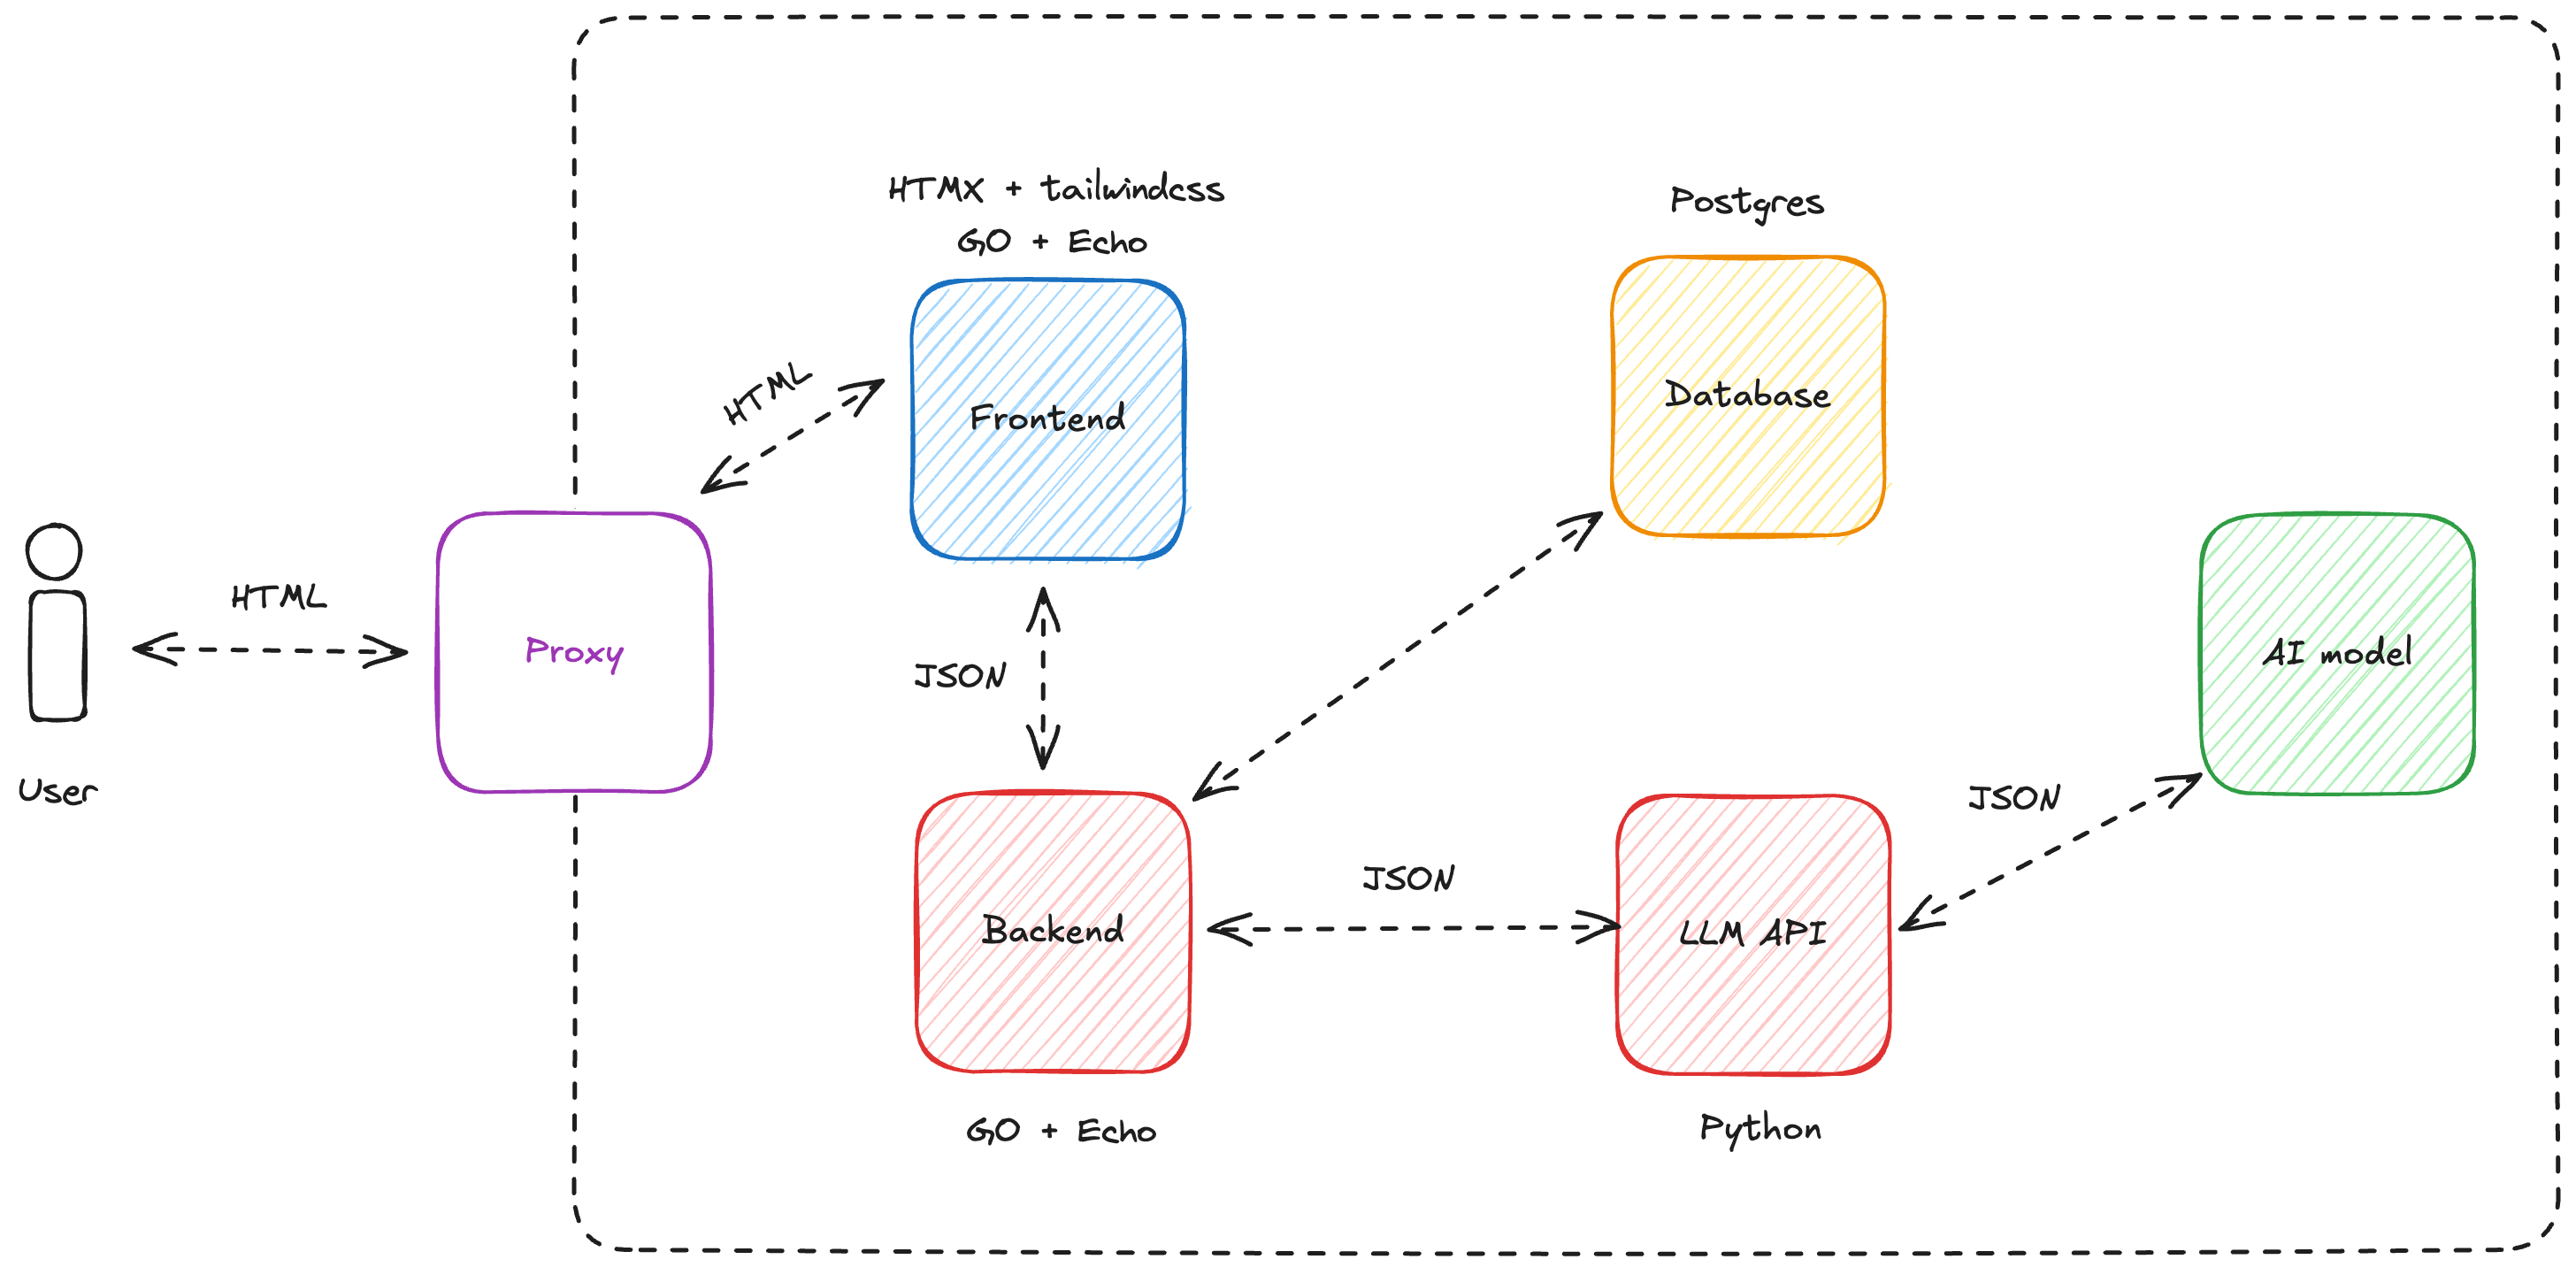
\includegraphics[width=0.9\textwidth, keepaspectratio]{figures/high-level-architecture.png}
    \caption{High-level system architecture}
    \label{fig:high-level-architecture}
\end{figure}

The frontend server is the part of the platform that users interact with directly. It's built as a server-rendered HTMX application using the Go programming language and the Echo framework. As the main entry point to the platform, it processes user inputs, communicates with the backend service, and provides content to users.

The backend is also written in Golang using the Echo framework. It is a regular REST application that communicates with HTTP requests. It brings together the different parts of the application and is responsible for the platform's business logic.

The database is Postgres, a popular, open-source relational database software. It stores all the data so the platform can work seamlessly. This component only communicates with the backend service.

The LLM API component is a unified interface for accessing the AI model. It is a small Python web application with a REST interface for more accessible communication. It contains prompts and question generation-related business logic. The component enables the platform to integrate different AI models and change between them.

The AI model component is a small application containing the question generator LLM. Máté Debreczeni fine-tuned the pre-trained \texttt{llama-3-8B-instruct} model for the platform on a custom dataset he created from Wikipedia articles \footnote{https://en.wikipedia.org/wiki/Wikipedia:Vital_articles} and questions generated by \texttt{gemini-1.5-flash}\footnote{https://deepmind.google/technologies/gemini/flash/} the fastest model of the Gemini family. He aims to train a model that combines the speed of \texttt{llama-3-8B-instruct} and the quality of questions generated by \texttt{gemini-1.5-flash}.

\subsection{Example component interaction}

Figure~\ref{fig:component-interaction} shows an example interaction between the components through a question generation. This interaction is the primary interaction between the components and utilizes all of them.

\begin{figure}[!h]
    \centering
    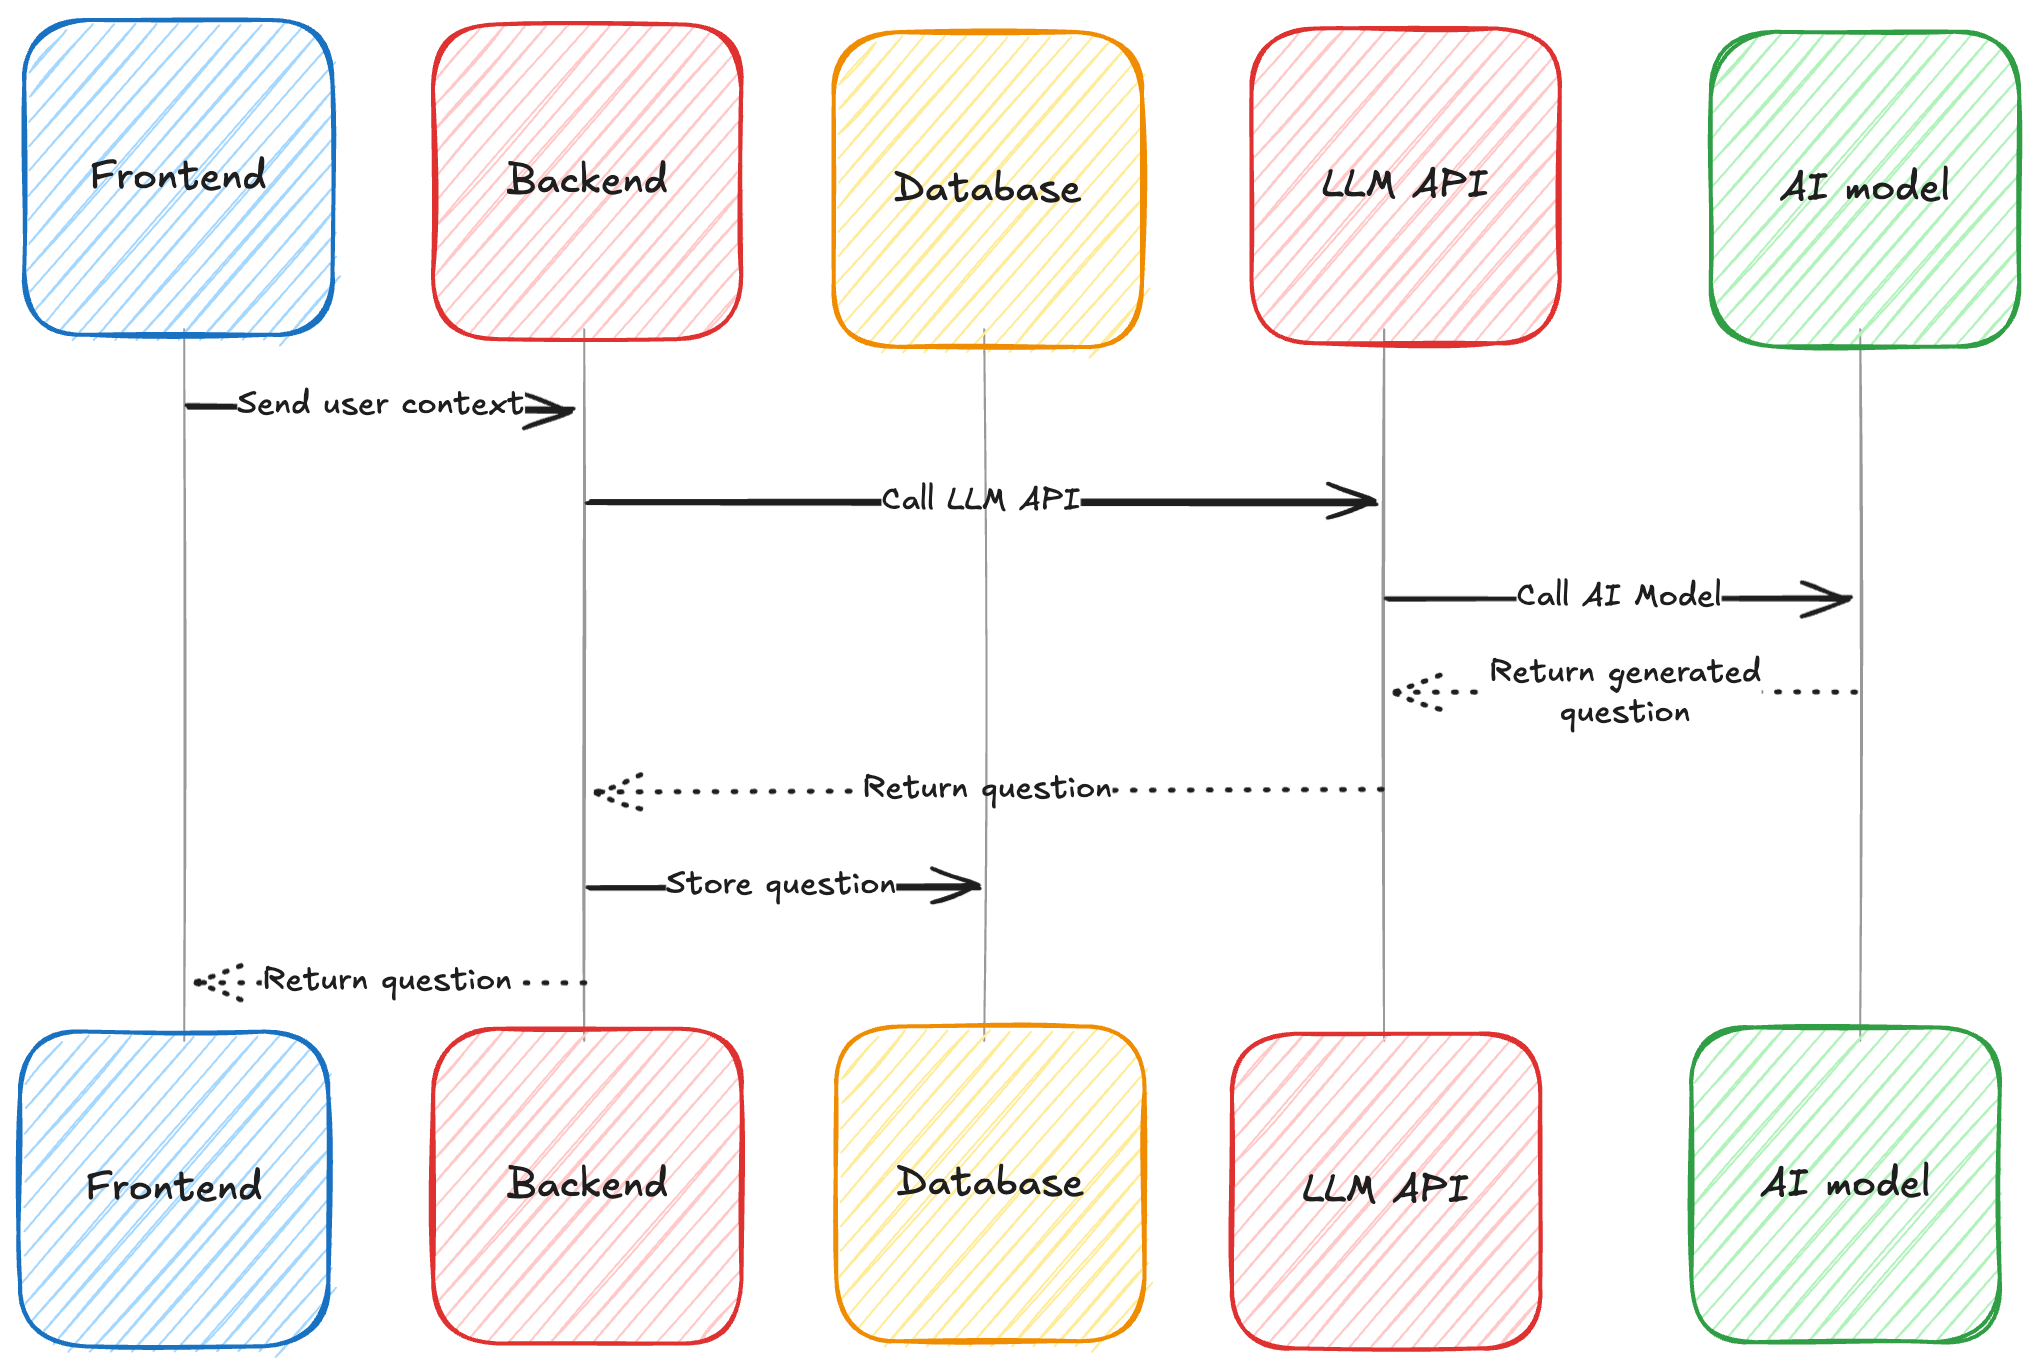
\includegraphics[width=0.85\textwidth, keepaspectratio]{figures/component-interaction.png}
    \caption{Component interaction: Question generation}
    \label{fig:component-interaction}
\end{figure}

Users submit their context to the frontend server, which validates the input and sets parameters like question type and quiz ID. The frontend calls the backend's proper endpoint with these parameters. The backend also validates the request and calls the LLM API to generate the question. The LLM API delegates the generation to the AI model through a request containing a pre-created prompt. This question is returned to the backend, where additional data is added and saved to the database. Finally, the backend returns the question to the frontend for display to the user.

\subsection{Deployment design}

Containerization is a crucial part of platform development and deployment. From the start, all the components were containerized with Docker for easier development and to ensure they worked on other machines. Máté worked on the AI model and the LLM API, and I worked on the other parts. Both of us used different operating systems, software, and tools. Without this method, we could not have worked together as efficiently as we did.

We created a Dockerfile for each service that describes how to build and run the respective application. We configured a docker-compose file to make them work together. We also considered building containers efficiently using the multi-layered containerizing approach. This idea was essential for the frontend and the backend due to the code generation, which has to be performed frequently.

\subsubsection{Development deployment}

Figure~\ref{fig:dev-deployment} shows how we deployed locally the platform for development. It consists of two groups: the local environment and the external environment. The local environment has all of the components in the system architecture diagram; this is a complete system. In comparison, the external environment consists of only one service, an LLM from Google. It is the company's fastest Gemini model called \textt{gemini-1.5-flash}.

The LLMs, even these smaller ones, need a lot of resources. Thus, question generation usually takes over a minute on a personal computer without a GPU. We sped up the development process using Gemini's API when developing and testing the services.

\begin{figure}[!h]
    \centering
    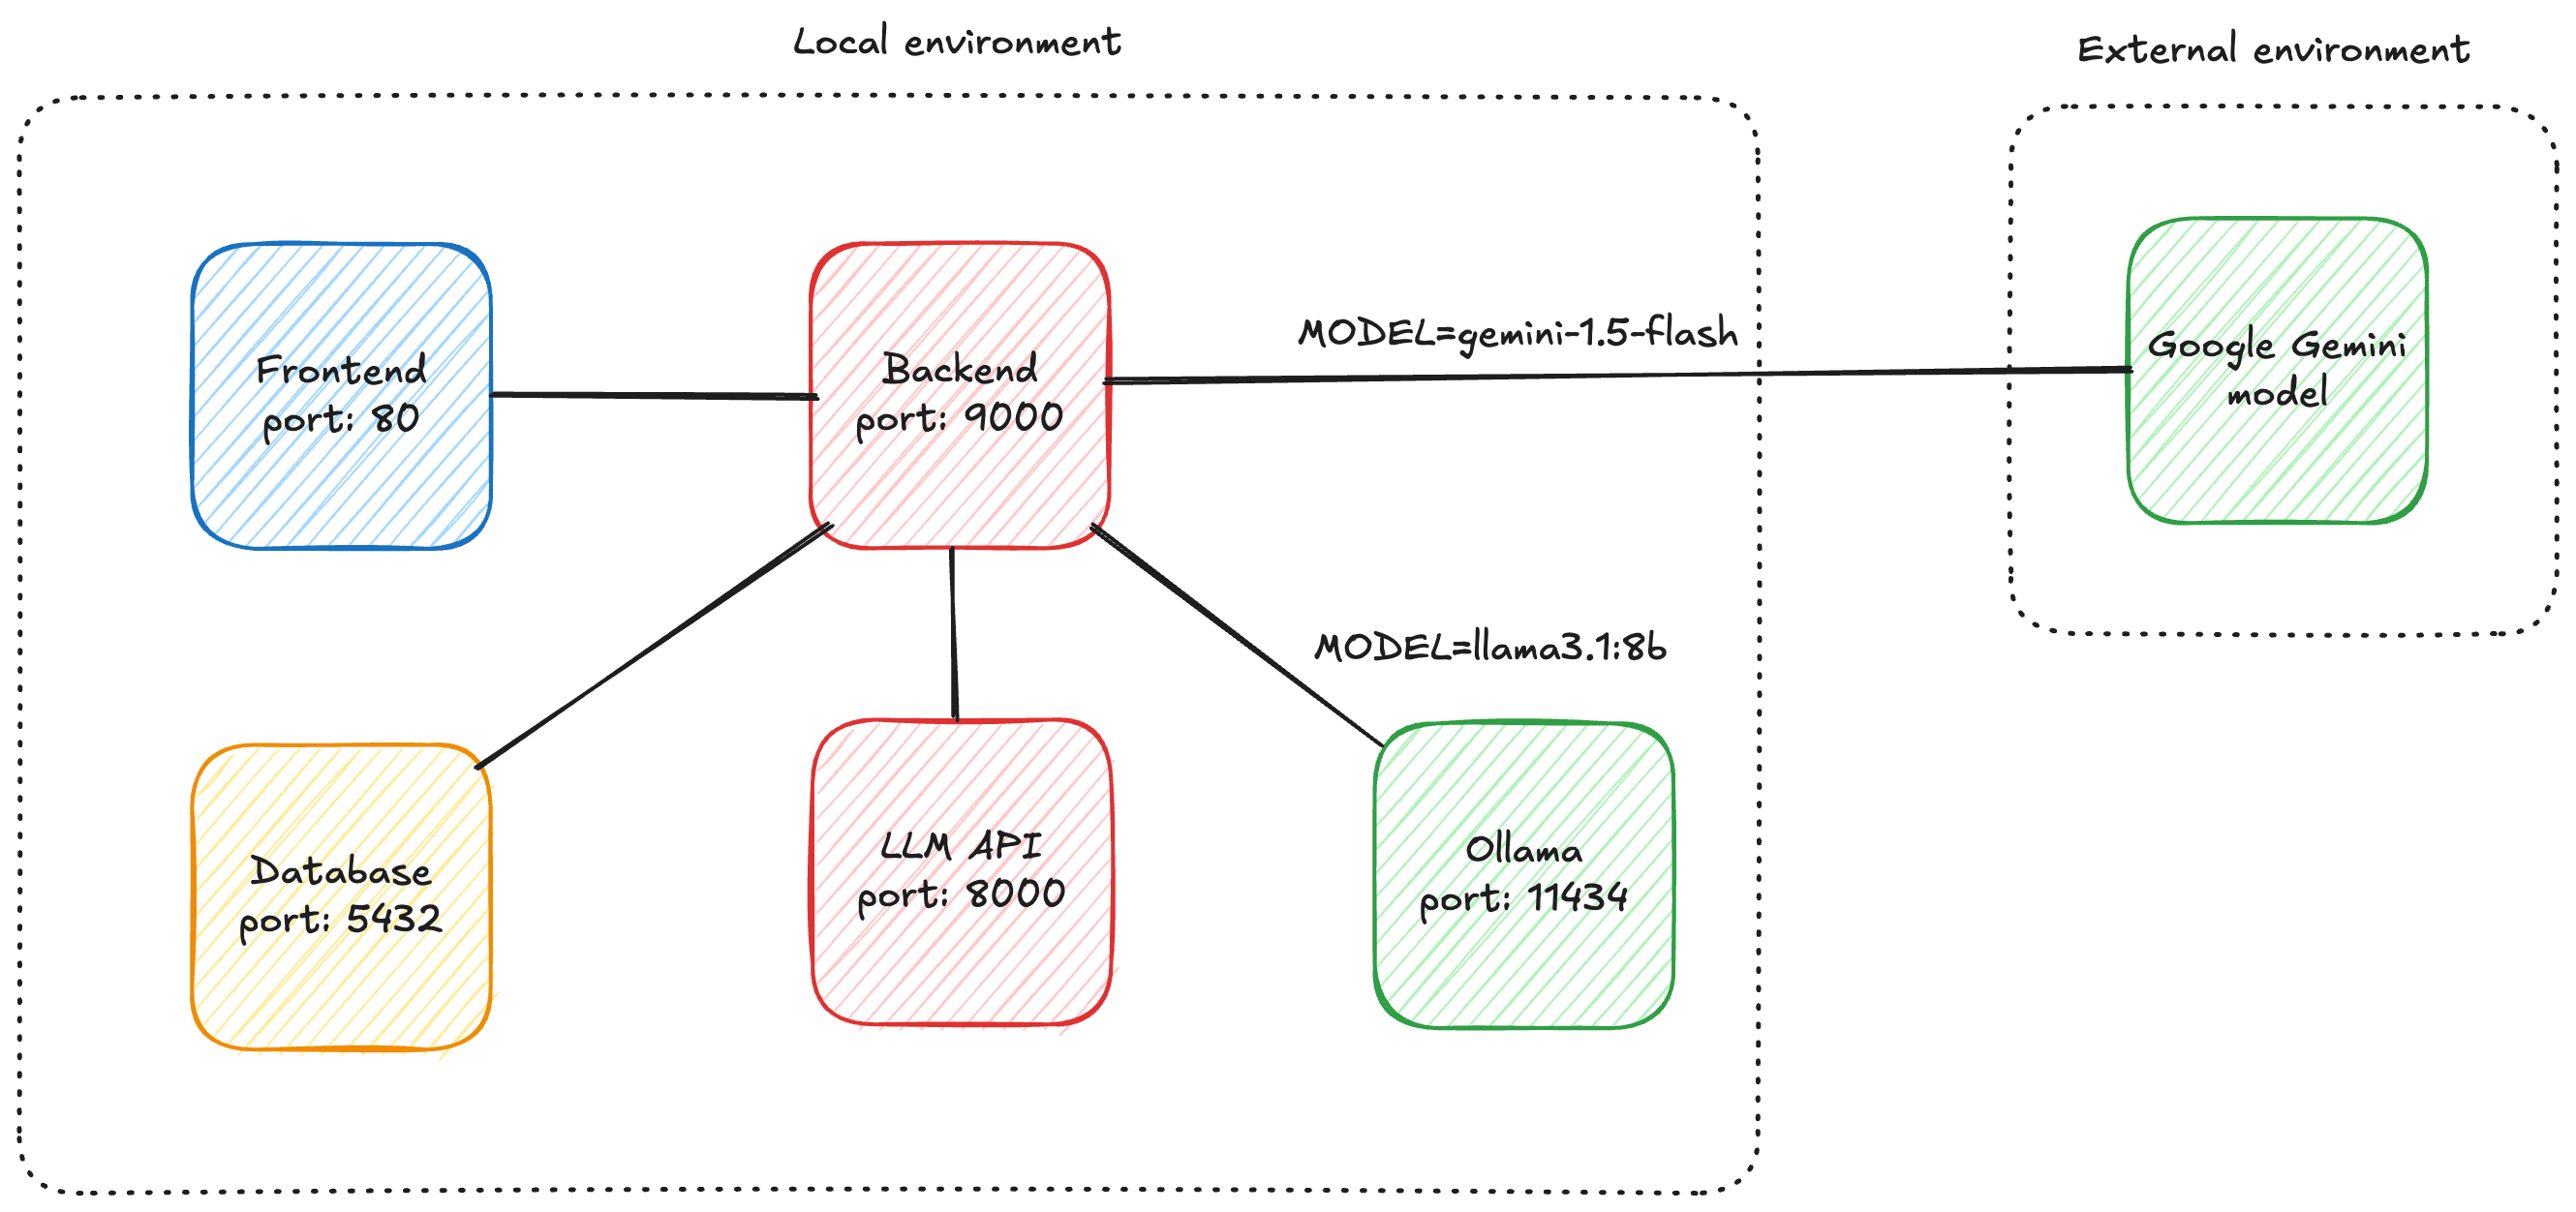
\includegraphics[width=0.9\textwidth, keepaspectratio]{figures/dev-deployment.png}
    \caption{Developer deployment}
    \label{fig:dev-deployment}
\end{figure}

\subsubsection{Production deployment}

We use a similar structure for production but without the Gemini model. We also split up the parts in this case into two, as Figure~\ref{fig:production-deployment} shows. The regular services (frontend, backend, database, LLM API) are found on Máté's VPS (Virtual Private Server) in a Kubernetes\footnote{https://kubernetes.io/} cluster, while the AI model is deployed to an external provider, RunPod \footnote{https://www.runpod.io/}. The VPS has no GPU; thus, we selected a provider specializing in running LLMs.

\begin{figure}[!h]
    \centering
    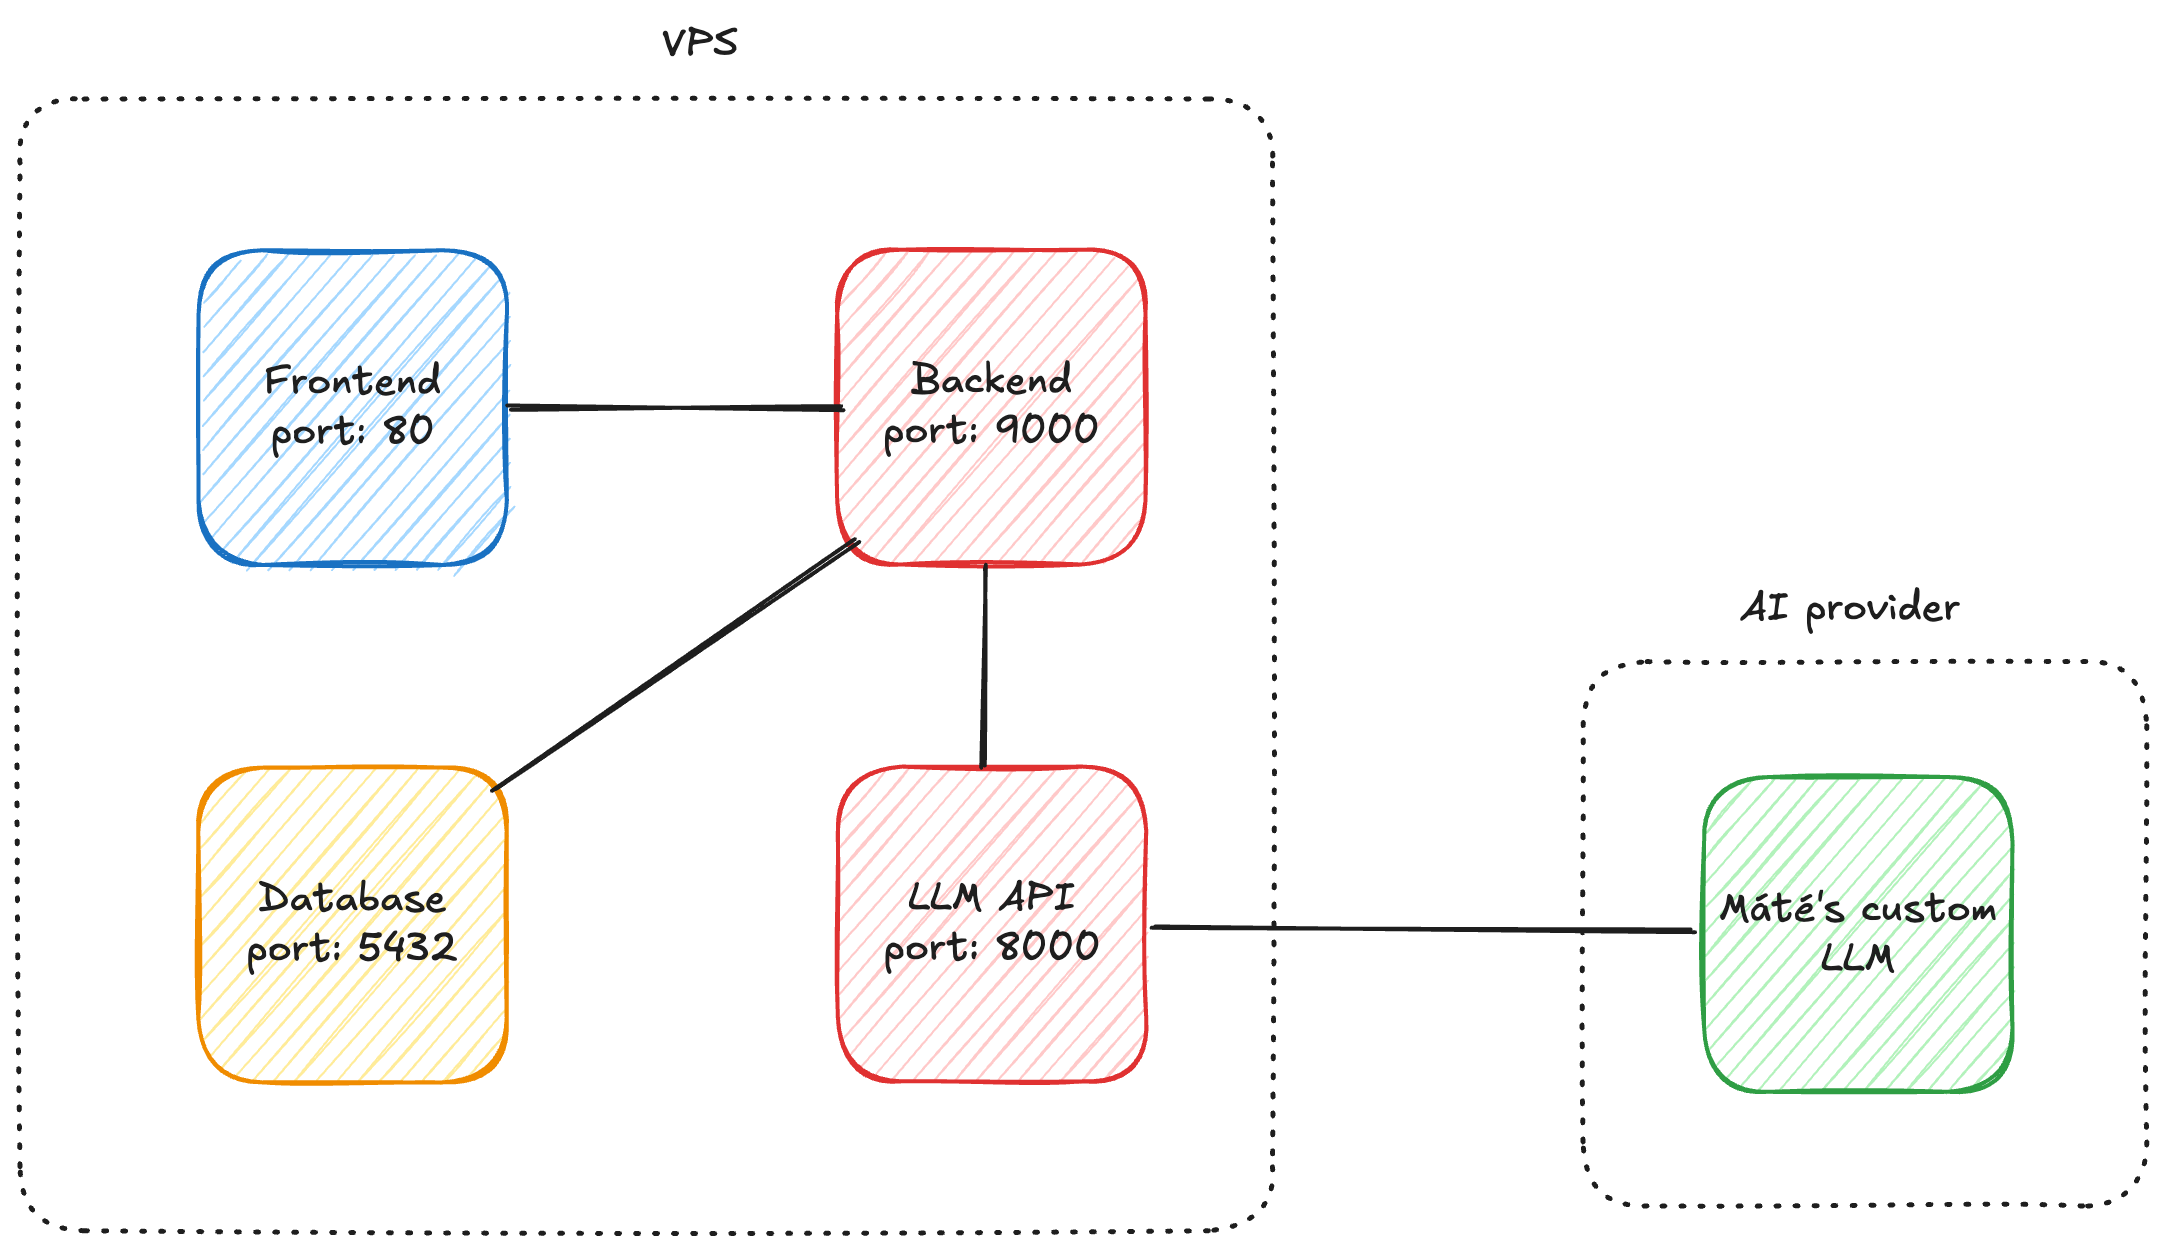
\includegraphics[width=0.9\textwidth, keepaspectratio]{figures/production-deployment.png}
    \caption{Production deployment}
    \label{fig:production-deployment}
\end{figure}

\section{Database Design}

Database design and software selection are critical parts of every web application; the same applies to the platform. Thus, we chose a relational database, Postgres, to store and serve the platform's data. I write about the database software selection and its rationale after introducing the data model from multiple aspects and the decisions behind them.

\subsection{Database software selection}

Postgres is one of the most popular Database Manager System (DBMS) software available today. It is free and open-source and offers a ready-to-use solution as a Docker container. We have worked with it for different projects through the years, and it has always been a good choice. So, its familiarity and reliability were the most important reasons for selecting it, besides its performance and wide adaption at database providers. 

Although it is a traditional database, it is extendable with third-party extensions. Its package manager is called trunk\footnote{https://pgt.dev/}, and it is effortless to install database packages by using it. We installed pgvector\footnote{https://github.com/pgvector/pgvector} for vector database features for the AI and another one called pgchron\footnote{https://github.com/citusdata/pg_cron} for scheduling session-related tasks.

\subsection{Entity-Relationship diagrams}

This section discusses the entities and their relationships in the application at this layer. I split it up into six smaller parts for easier understanding and overviewing.

\subsubsection{Users and sessions}

The database has two entities tightly connected to the user: User and Session. The User entity holds regular information about the user, like name, email, and hashed password, while the session stores the current user's session and its validity. When the user authenticates, a session is created and sent to the user's computer as a session cookie for later use. The session ID is used for authentication throughout the whole platform and has an expiration date when a pgchron task automatically deletes it. Figure~\ref{fig:er-user-and-session} displays the entities and the relationship between them.

\begin{figure}[H]
    \centering
    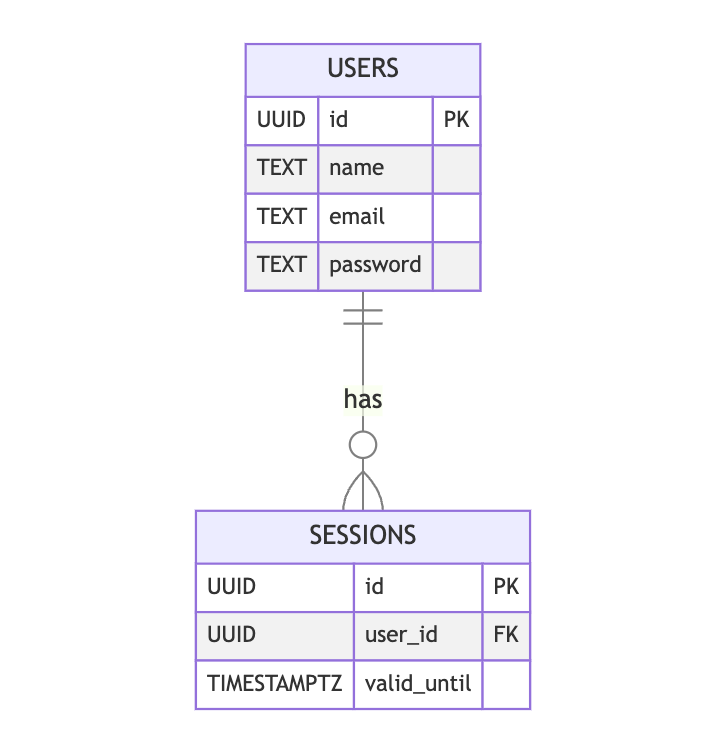
\includegraphics[width=0.8\textwidth, keepaspectratio]{figures/er-user-and-session.png}
    \caption{ER Diagram: User and Session}
    \label{fig:er-user-and-session}
\end{figure}

\subsubsection{Quizzes and questions}

The platform's core entities are the Quizzes and their questions. Each quiz has a name, description, and creator and is linked to different types of questions. There are three types of questions: SingleChoiceQuestion, a question with only one correct answer; MultipleChoiceQuestion, which can have multiple correct answers; and TrueOrFalseQuestion, aka a boolean question. Each type has its entity and table in the database. They are mostly the same; they all have a more extended text field describing the question and differ in the answer type.

The quizzes can be accessed through a QuizAccess entity, which links the user to a quiz with a role. By default, an instance with an owner role is generated automatically when a user creates a quiz. This abstraction allows controlling which quiz can be viewed or edited by whom. It also makes it available for future development as a platform for sharing private quizzes or creating public ones. Figure~\ref{fig:er-quizzes} displays the quizzes, types of questions, and accesses in an ER diagram.

\begin{figure}[H]
    \centering
    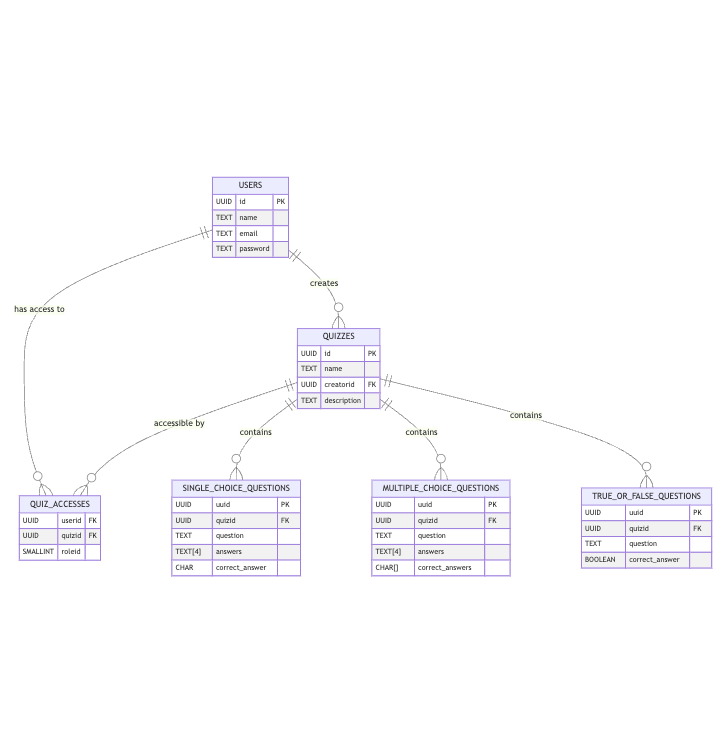
\includegraphics[width=0.9\textwidth, keepaspectratio]{figures/er-quizzes.png}
    \caption{ER Diagram for quizzes and questions}
    \label{fig:er-quizzes}
\end{figure}

\subsubsection{Quiz sessions}

Another essential entity category is related to answering questions. The central entity is the QuizSession, which holds the information together for quiz completion. It accounts for start and finish time and links to answers connected to questions. And it is also related to the quiz result if it is submitted. Some answer entities hold the information of the user's answer to the given question. Figure~\ref{fig:er-quiz-session} shows these relations.

\begin{figure}[H]
    \centering
    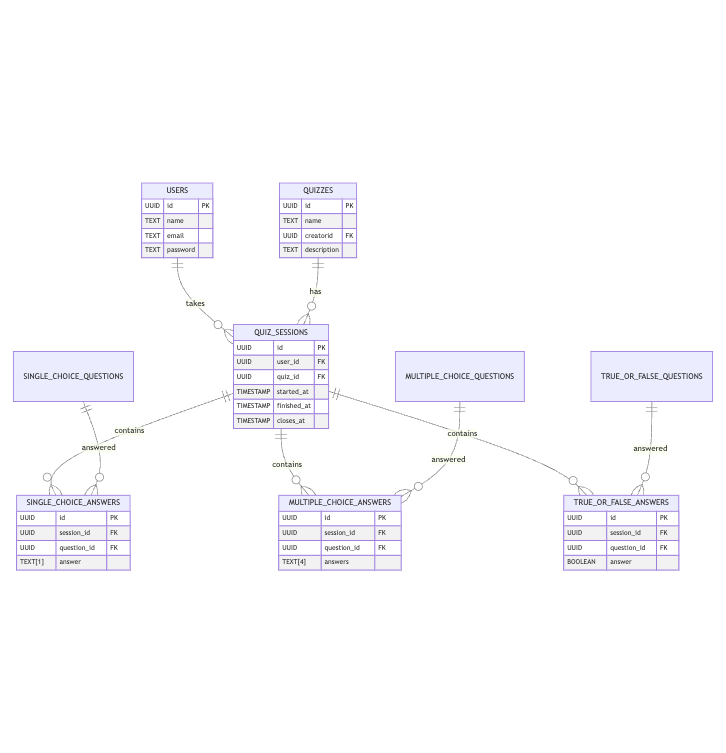
\includegraphics[width=0.9\textwidth, keepaspectratio]{figures/er-quiz-sessions.png}
    \caption{ER Diagram for quiz sessions}
    \label{fig:er-quiz-session}
\end{figure}

\subsubsection{Answers and quiz results}

In addition to the entities detailed before, there are more entities related to QuizSession, but now, it is for storing the scores for the answers and the results of the finished one. When a quiz is submitted and the session is finished, AnswerScore entities are created, which store the user's score for their given answers, and a question result record is also added with total scores. QuizResult is just a supporting entity for later extensibility capabilities; currently, it could have been merged into the QuizSession. 

\begin{figure}[H]
    \centering
    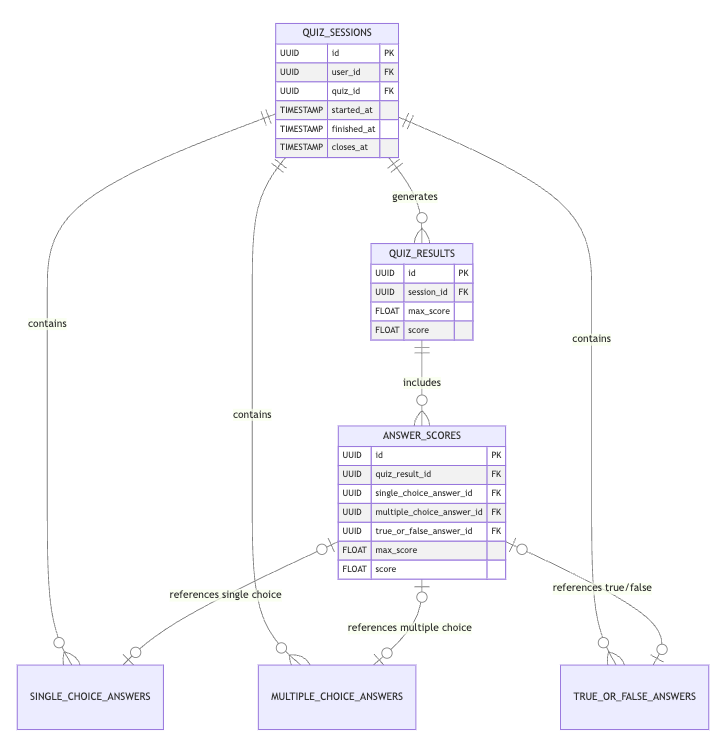
\includegraphics[width=0.9\textwidth, keepaspectratio]{figures/er-quiz-result.png}
    \caption{ER Diagram for answers and quiz results}
    \label{fig:er-quiz-result}
\end{figure}

Each AnswerScore has a max\_score and score field, which holds the maximum available and the obtained score. It establishes three distinct relationships corresponding to different question types. These relationships are structured with cardinality constraints, ensuring that a single AnswerScore can be linked to only one question at a time, maintaining a one-to-zero or one-to-one connection depending on the specific question type. Figure~\ref{fig:er-quiz-result} shows all the entities and relations mentioned in these paragraphs.

\subsubsection{Learning list}

LearnListAddedItem is a small entity that links the users to the quizzes they decided to start learning with the spaced repetition algorithm. When a LearnListAddItem is inserted, the platform automatically creates and schedules ReviewItem entities for each quiz question with initial learning parameters. Also, by removing a learn list item, the ReviewItems are deleted. Figure~\ref{fig:er-learn-list} shows the connection between the user and the selected quizzes in the context of a learning list.

\begin{figure}[H]
    \centering
    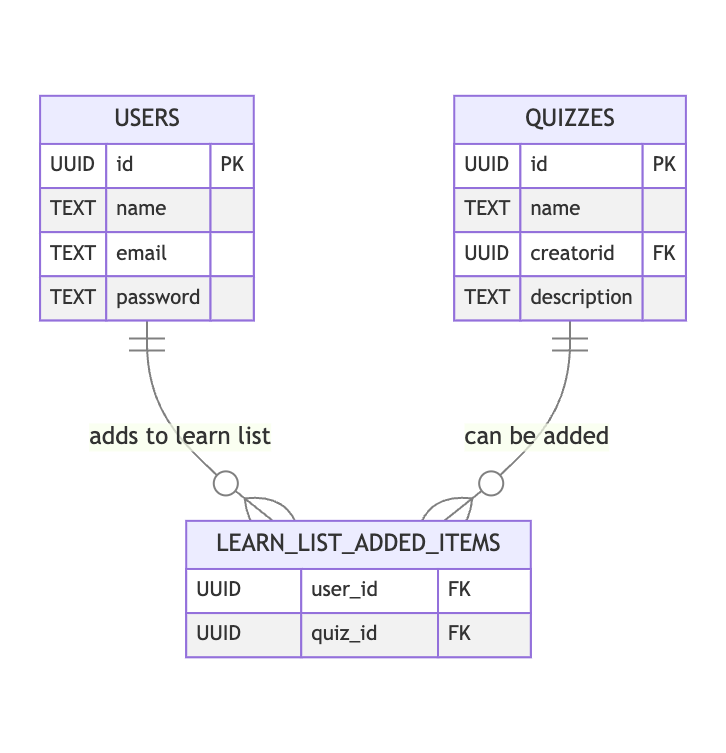
\includegraphics[width=0.9\textwidth, keepaspectratio]{figures/er-learn-list.png}
    \caption{ER Diagram for learn list}
    \label{fig:er-learn-list}
\end{figure}

\subsubsection{Review items}

The ReviewItem item is the core entity of the spaced repetition algorithm. When the user adds a quiz to its learning list, one instance is created and scheduled for learning immediately for each question. A ReviewItem is always linked to the user; each relation includes strictly one question. Figure~\ref{fig:er-review-items} shows these relations.

\begin{figure}[H]
    \centering
    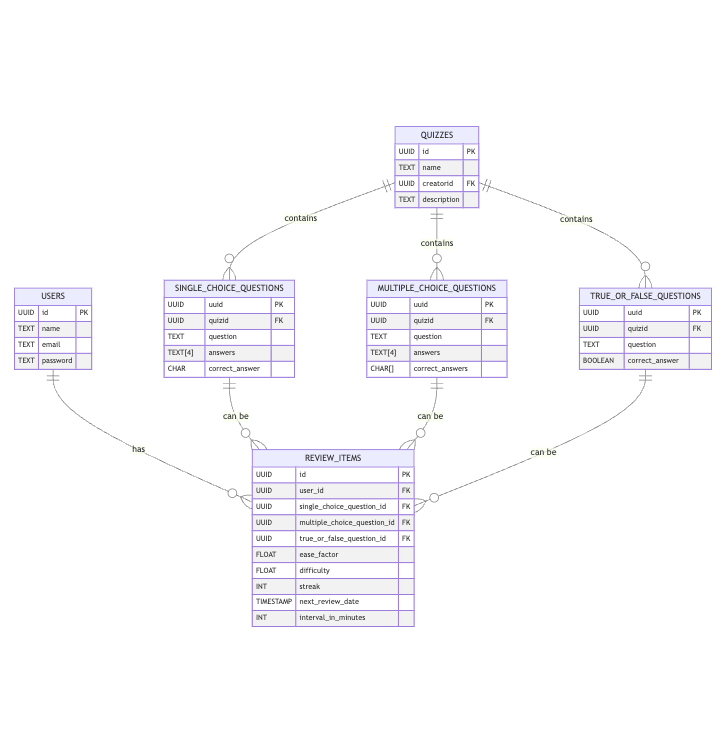
\includegraphics[width=0.9\textwidth, keepaspectratio]{figures/er-review-items.png}
    \caption{ER Diagram for review items}
    \label{fig:er-review-items}
\end{figure}

It holds all the information the learning algorithm uses to determine the next review date. It has fields for the ease factor, the difficulty, and the user's correct answer streak. It also contains the learning interval time and the next review date. The spaced repetitions algorithm determines and controls all the information based on the user's answers and the previous values of the ReviewItem.

\subsubsection{Data type selection}

The primary rationale behind selecting the data types was to minimize storage usage and optimize performance. Regardless of this, most variables have NON-NULL constraints wherever possible to avoid handling these cases on the backend side. In the cases where NULL values are allowed, they have a particular purpose. For example, the answer entities' answer fields with NULL values mean the user did not answer them. The selected data types can be grouped into the following categories: identifiers, numbers, texts, and time.

The Postgres database offers numeric and UUID-based data types for identifying records. We initially decided to use the UUID fields as identifiers because they are usable across different services. It was a good idea because it worked, but it needed some configuration for the code generation in the database library on the backend side. However, we only used one database for the whole system. Thus, the advantages over the numeric IDs were negligible.

Although the database offers several numeric\footnote{https://www.postgresql.org/docs/current/datatype-numeric.html} types, the platform only needed a few of them. The role ID was a small int, which is a 2-byte long integer number, and that was more than enough because it's like an enum with very few possible values. The correct answer streak and learning interval were INT types, as they can have slightly larger values over time. In addition, non-integer numbers were needed in some places, e.g., score, max\_score, ease\_factor, and difficulty; here, the database's FLOAT type is used.

We chose the most straightforward to use for textual fields, the unlimited-length text, also called text. It could be more efficient, but these fields are primarily used for reading in one piece, not searching.

Time synchronization between components is a must for even small systems. Proper date and time type selection is the bedrock of this. We chose the timestamp type, which is the most detailed representation of time in 8 bytes and is supported by most frameworks and libraries. However, the platform needed some configuration because of Go's nil-handling approach. One challenge was creating and parsing it correctly to be processed and displayed. This type was used for the user sessions, quiz sessions, and learning algorithm scheduling.

\subsubsection{Indexing strategy}

A reasonable indexing strategy can boost a database's performance, accelerating its other components. However, a poor strategy could have the opposite effect on a system. Our indexing strategy was to create an index to reduce the overall execution time on columns affected by the queries' WHERE clauses or table JOINs. These columns were UUID types in almost all cases, and timestamps were used only once in the question session table.

\subsubsection{Constrains and integrity rules}

System integrity is one of the most critical requirements, if not the most vital. Proper settings and rules can enforce it. To keep the database consistent, we used these additional constraints: ON DELETE CASCADE, UNIQUE, and CHECK. The first one ensures that when a record is deleted, all the records in other tables referring to it are also deleted. The UNIQUE was used to avoid inserting a record already in the table again. Finally, the CHECK was used in the ANSWER\_SCORES and REVIEW\_ITEMS tables to prevent multiple questions from being linked to them. Listing~\ref{lst:db-check-constraint} shows an example using the CHECK constraint on the ANSWER\_SCORES table.

\begin{lstlisting}[caption=Using CHECK constraint,label=lst:db-check-constraint]
CREATE TABLE IF NOT EXISTS answer_scores(
    id UUID PRIMARY KEY NOT NULL,
    quiz_result_id UUID REFERENCES quiz_results(id) ON DELETE CASCADE NOT NULL,
    single_choice_answer_id UUID REFERENCES single_choice_answers(id) NULL,
    multiple_choice_answer_id UUID REFERENCES multiple_choice_answers(id) NULL,
    true_or_false_answer_id UUID REFERENCES true_or_false_answers(id) NULL,
    CHECK (
        (single_choice_answer_id IS NOT NULL)::int +
        (multiple_choice_answer_id IS NOT NULL)::int +
        (true_or_false_answer_id IS NOT NULL)::int = 1
    ),
    max_score FLOAT NOT NULL,
    score FLOAT NOT NULL
);
\end{lstlisting}

\section{Frontend Design}

Designing an application's front end is as important as planning the other parts because this is what the user sees and uses. To make the user like the platform, we must create a good-looking and good-working frontend application. This section outlines how the design is created, how the components are structured, and the most important goals when I designed the platform's interface.

\subsection{User Interface design principles}

\subsubsection{Chosen design methodology}

The frontend design methodology follows a minimalist, modern approach similar to shadcn/ui\footnote{https://ui.shadcn.com/}, a UI component collection popularized by Vercel\footnote{https://vercel.com/} made for React and other web frameworks. The application does not use these components and styles because HTMX is not supported directly. Still, their source code is publicly available, and these components are made to copy-paste and customize later. It served as a good starting point for the application's methodology.

shadcn/ui is a collection of beautifully designed reusable UI components for web applications. They have a very minimal style and color selection because the creator made them to be customized by the developers. However, these components look good in reality by default, and most small applications and MVPs do not require an extraordinary design; the developers started using them as they are, and others kept following them until they became viral in 2024. Figure~\ref{fig:shadcn} shows some of these components.

\begin{figure}[H]
    \centering
    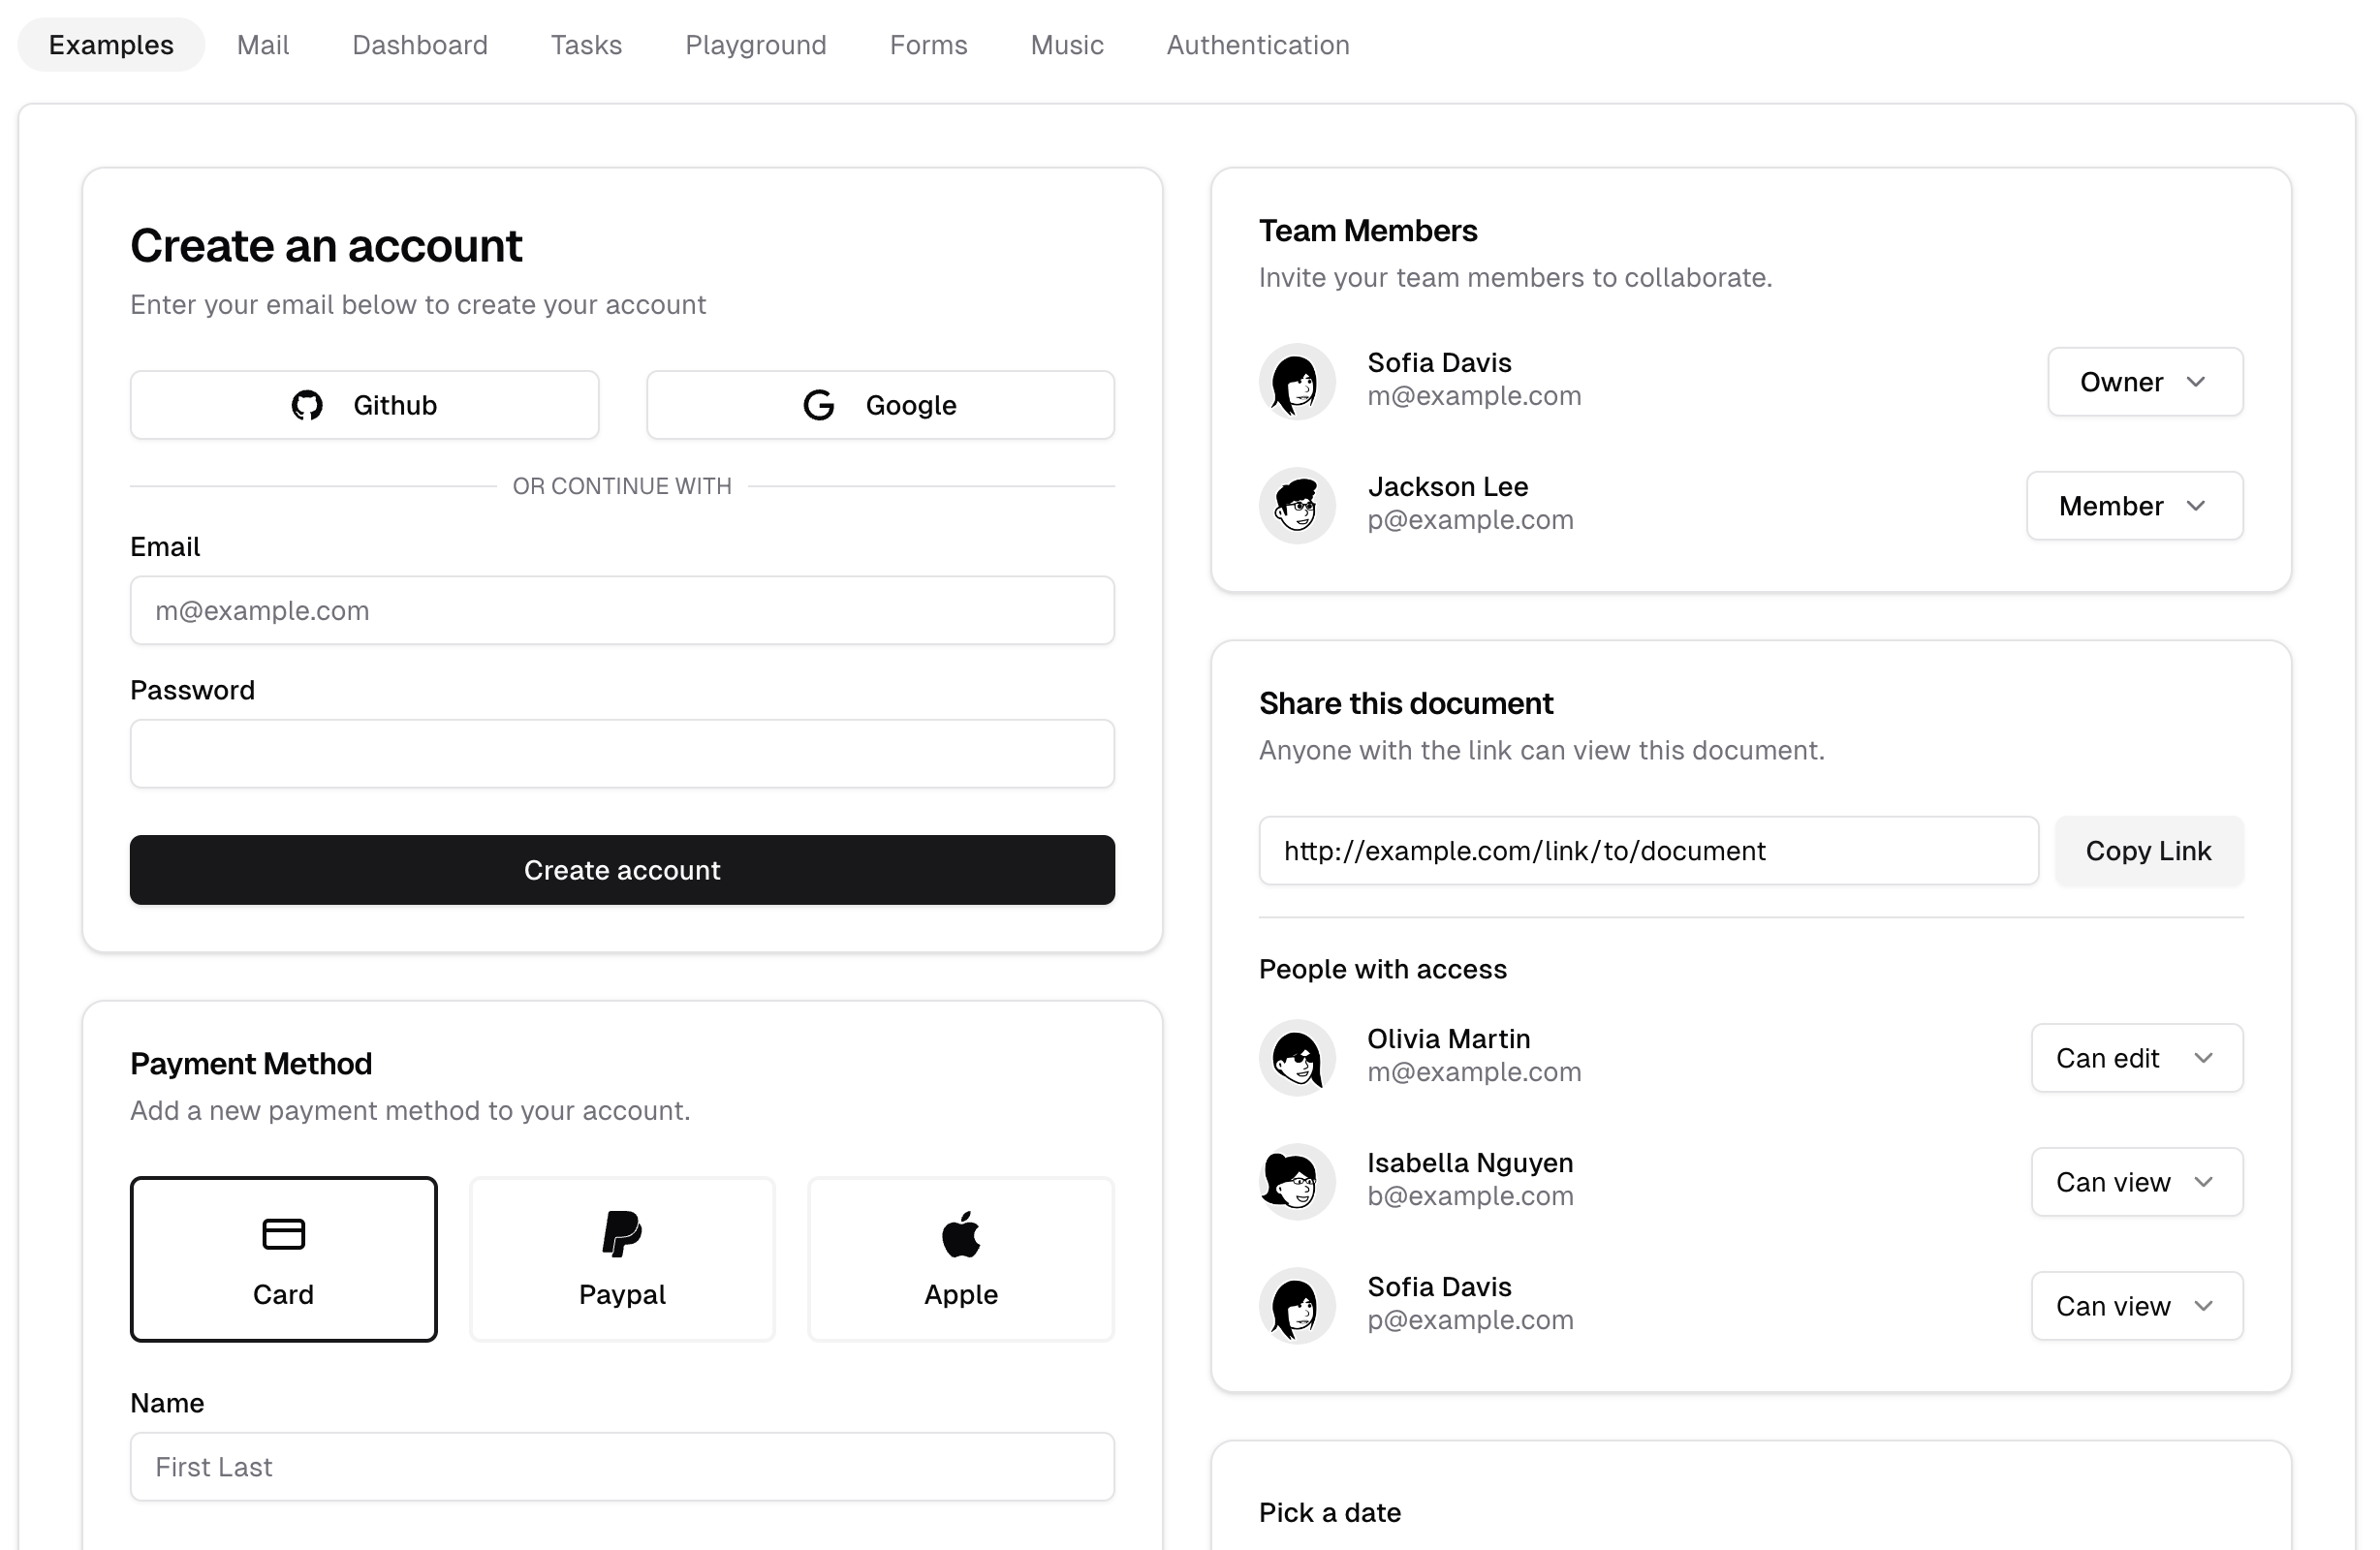
\includegraphics[width=0.8\textwidth, keepaspectratio]{figures/shadcn-example.png}
    \caption{shadcn/ui components example, Source: https://ui.shadcn.com/examples/cards}
    \label{fig:shadcn}
\end{figure}

An alternative approach could have been Google's Material Design\footnote{https://m3.material.io/}, another popular option. It is used in almost every Google product and supports various frameworks, including Android applications. It is battle-tested because its first version was released 10 years ago and underwent significant redesigns, but it always stayed well-welcomed. Figure~\ref{fig:material3} shows an example of their current version (Material 3). While they are designed well, and their components look consistent across different platforms, they are not easily customized and used outside the supported frameworks.

\begin{figure}[H]
    \centering
    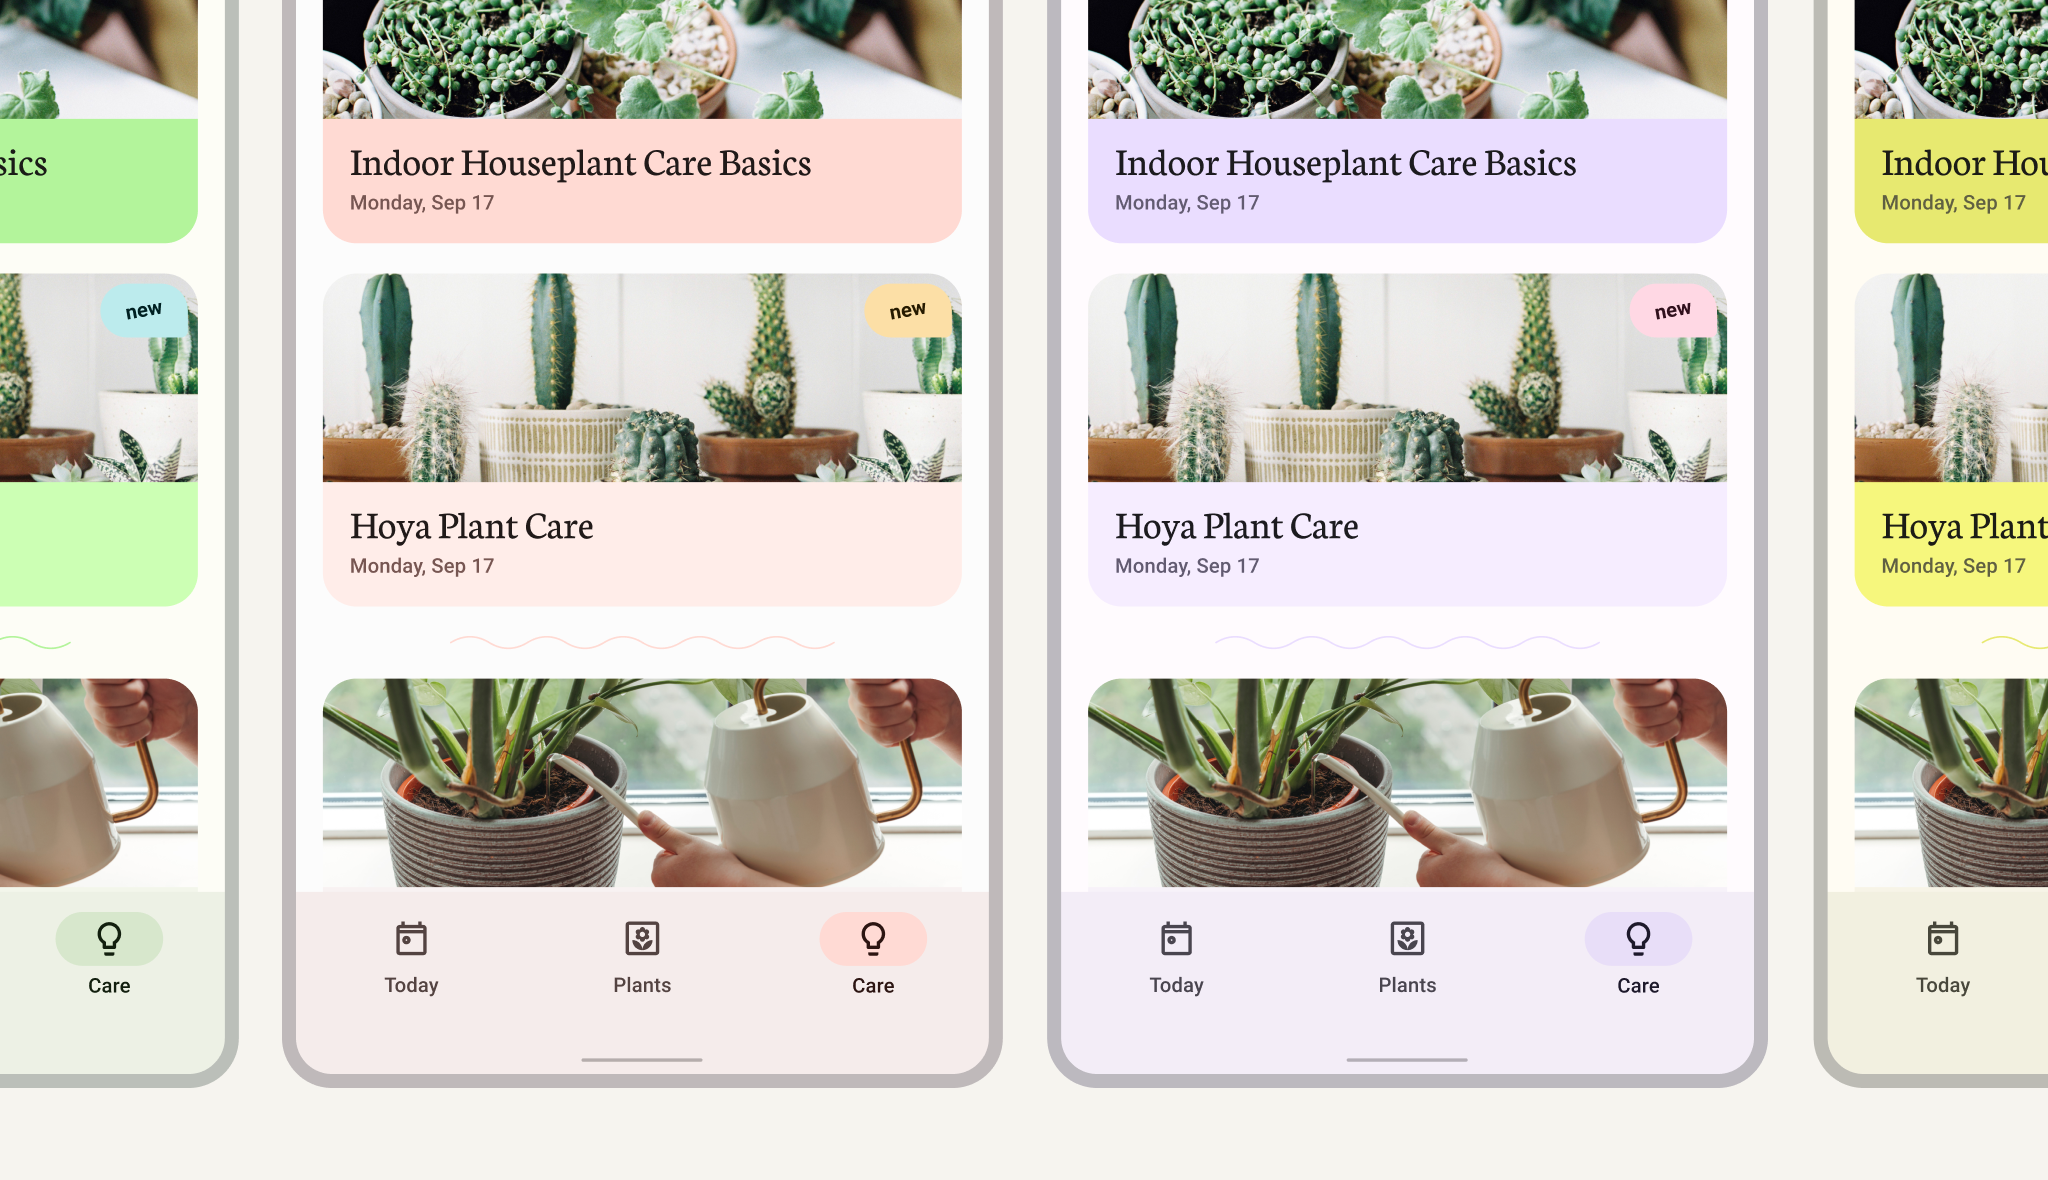
\includegraphics[width=0.8\textwidth, keepaspectratio]{figures/material3.png}
    \caption{Material 3 design for Android applications, Source: https://m3.material.io}
    \label{fig:material3}
\end{figure}

\subsubsection{User experience principles and goals}

To create an enjoyable user experience, we must consider some user experience (UX) principles, as outlined in~\cite{cooper2014face}. Users are diverse, with a wide range of needs and backgrounds, but we must design interfaces that suit most users. This involves adopting design practices prioritizing clarity, accessibility, responsiveness, and intuitiveness. The following principles and goals guided the development of the frontend application:

\begin{itemize}
\item \textbf{Clarity and simplicity}: The application's interface should communicate clearly and avoid unnecessary complexity.
\item \textbf{Accessibility}: The application should be inclusive for the broadest range of users. This means the design should consider alternative navigation options, support screen readers, and use appropriate contrast. For the platform, I did not have enough time to focus on this, but the keyboard can use some of the features, and the colors comply with contrast requirements as they are from the tailwindCSS's color palette. In the future, this is an aspect for the platform point to improve and an excellent opportunity to reach more users.
\item \textbf{Consistency}: Consistency ensures a seamless experience across the application, encompassing the design, behavior, color schemes, and typography of its elements. In my personal opinion, consistency is one of the most fundamental aspects of software design, influencing not only the application's look and feel but also its underlying code and architecture.
\item \textbf{Feedback}: The user should see feedback immediately after the interaction. This ensures the user is informed about the performed action and helps the user understand what is happening. This can be achieved by adding an interactive state for the elements on hover or click, showing loading indicators, and showing success or error messages with the performed action.
\end{itemize}

\subsubsection{Technology stack selection}

I chose a technology stack that supports the described design methodology and gives a breath of fresh air by using something other than well-established web frameworks. That is why I created the platform using HTMX and Go. For styling the platform, I used tailwindcss \footnote{https://tailwindcss.com/}, a utility-first CSS library instead of plain CSS. It supports rapid prototyping and development and features a versatile pre-defined color palette perfect for websites with a modern minimalist design.

HTMX is a lightweight JavaScript library that enables declarative HTTP requests via HTML attributes, inserting HTML fragments from the response directly into the DOM. This extension of HTML functionality provides interactivity comparable to modern client-side frameworks. HTMX runs on the user's browser, while the server can use any technology compatible with the HTTP protocol. Table~\ref{tab:htmx-vs-others} summarizes the difference between HTMX and traditional SPA frameworks.

\begin{table}[H]
    \centering
    \resizebox{\columnwidth}{!}{%
    \begin{tabular}{|l|c|c|} \hline
        \textbf{Characteristic} & \textbf{HTMX} & \textbf{traditional SPA frameworks} \\ \hline
        Rendering approach & Server-side rendering & Client-side rendering \\ \hline
        Supported technologies & Any HTTP protocol compatibly technology & JavaScript and TypeScript \\ \hline
        State management complexity & Lower & Higher \\ \hline
        Client-side JavaScript code complexity & Low or even zero & Higher \\ \hline
        Performance & Lighter and faster initial loads & Heavier initial load \\ \hline
        Tooling & Lack of tools & Extensive set of supported tools \\ \hline
        Use case & Content-driven sites with minimal interactions & Complex, state-heavy application  \\ \hline
    \end{tabular}%
    }
    \caption{HTMX vs. traditional SPA frameworks}
    \label{tab:htmx-vs-others}
\end{table}

\subsection{Architecture planning}

\subsubsection{Selected frontend architecture pattern and rationale}

For the frontend application, I opted for a component-based architecture. This approach involves breaking down the user interface into smaller, reusable components, like other modern web frameworks, such as React. "The breaking down of a user interface into smaller, self-contained components allows for modularity and reusability across codebases. Through this approach, one gets easier maintenance and scalability for an application, along with better separation of concerns, thereby allowing teams to work more effectively in parallel."\cite{Kothapalli2021ComponentBased}. I used a combination of HTMX, templ, and tailwindCSS to implement this architecture. This approach offers several advantages I think are important for the platform:

\begin{itemize}
\item \textbf{Modularity}: The components are self-contained units of functionality, making it easier to develop and maintain smaller application pieces.
\item \textbf{Reusability}: Components can be reused in different application parts, reducing redundant code.
\item \textbf{Scalability}: Adding more components to the application has minimal impact on the overall performance.
\item \textbf{Parallel development}: Different teams can work on the components simultaneously.
\item \textbf{Improved testing}: These components can be tested independently, making the application more robust.
\end{itemize}

\subsubsection{Component hierarchy planning}

To implement this architecture, I established a hierarchical structure of components. This hierarchy also helps manage and organize the application code. These components can be categorized into top, mid, and low.

As their names suggest, the top-level components are the most important ones. They create an essential layout structure of the pages and contain the lower-level ones. These are the following:

\begin{itemize}
\item \textbf{HTML layout}: This component is a root HTML document holding the HTML head and body. This component includes the required metadata and scripts to work the application. It also serves as a container for the pages and popups.
\item \textbf{Authenticated layout}: It is a container layout for pages available after authentication. It also contains a sidebar responsible for navigation between pages and quizzes.
\item \textbf{Navbar}: Navbar is a navigation helper component for the pages available before authentication.
\item \textbf{Sidebar}: Sidebar is also a navigation helper component for accessible pages for authenticated users. They offer similar functionality but are placed differently to separate the look and feel of the landing page and the application.
\end{itemize}

Figure~\ref{fig:top-level-components} shows an example structure using them.

\begin{figure}[H]
    \centering
    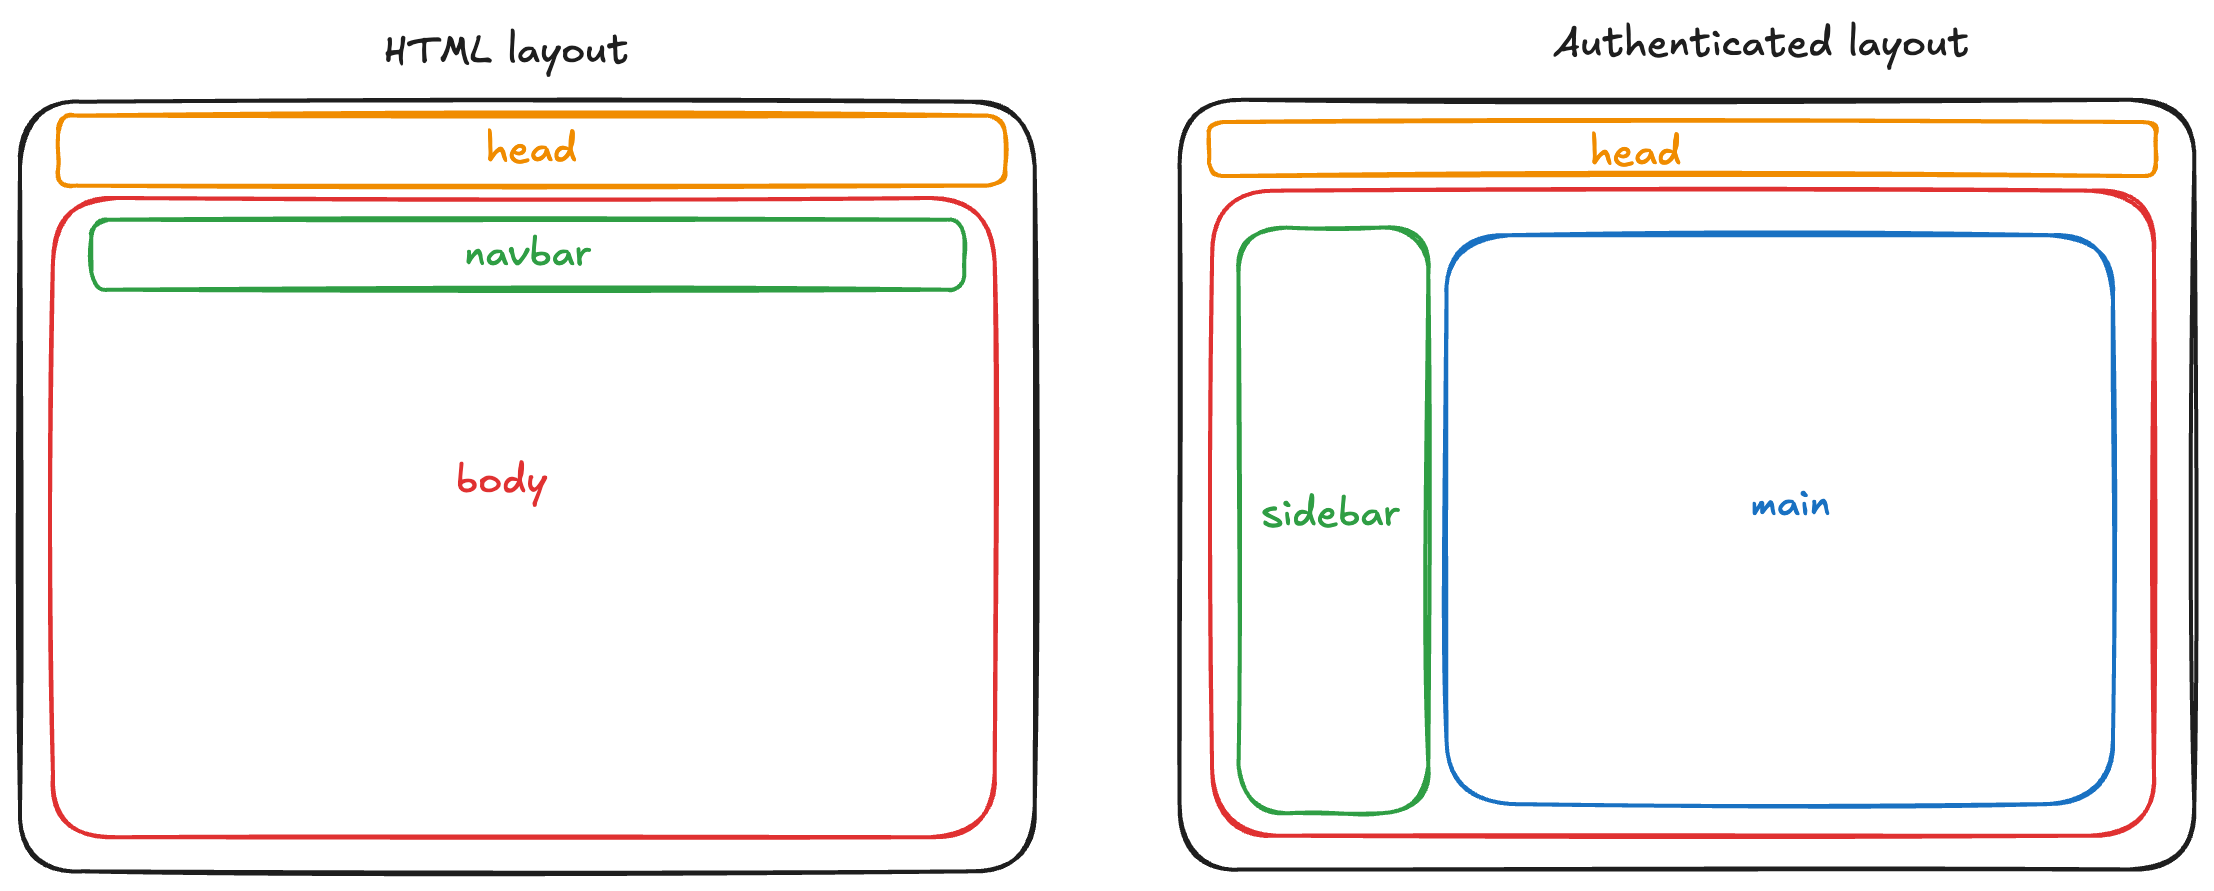
\includegraphics[width=0.8\textwidth, keepaspectratio]{figures/top-level-components.png}
    \caption{Top-level component}
    \label{fig:top-level-components}
\end{figure}

Mid-level components are also fundamental components for the whole. They usually correspond to a specific function that is used in multiple parts of the application. They are built and heavily rely on low-level components. These are a few of them: 

\begin{itemize}
\item \textbf{Quiz card}: On "My quizzes" page, there is a list of Quiz cards. Each quiz card has a short title and buttons for editing, deleting, and taking the related quiz.
\item \textbf{Learning list popup}: The learning list popup is available from the "My Quizzes" page to show. It helps manage the users which quiz they want to learn with the platform. It consists of a list of available quizzes and added quizzes to the learning list.
\item \textbf{Question}: Each question type has a Question component. These components have different modes with a similar look but extended behavior because they are used for editing and taking quizzes or reviewing their result.
\item \textbf{Review item}: Review item is a component used in the "Learn" page of the platform for listing the questions scheduled for review. A table row element displays questions, difficulty, review dates, and scores. It is built of smaller components such as text and buttons. Figure~\ref{fig:review-item-component} shows an example of a review item in the table.
\end{itemize}

\begin{figure}[H]
    \centering
    
\includegraphics[width=0.9\textwidth, keepaspectratio]{figures/review-item-component.png}
    \caption{Review item component}
    \label{fig:review-item-component}
\end{figure}

Low-level components are everywhere in the application, as they are the essential building blocks for other components. They consist of styles of text, different kinds of input fields, buttons, and other interactive elements. They are primarily wrappers over basic HTML DOM elements with customizable styles and extended functionalities. Figure~\ref{fig:low-level-component} shows an example of a styled text input field with a validation error.

\begin{figure}[H]
    \centering
    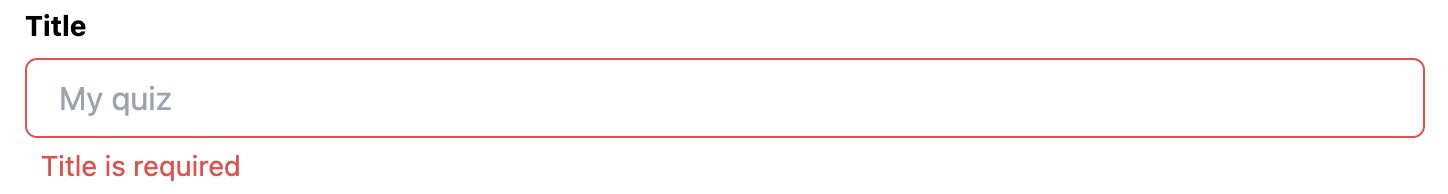
\includegraphics[width=0.8\textwidth, keepaspectratio]{figures/low-level-component.png}
    \caption{Low-level component: Text field containing a validation error.}
    \label{fig:low-level-component}
\end{figure}

\subsubsection{Routing and navigation structure}

The application's routing is simple and self-describing. All the pages are available directly through in-app navigation or URLs. The naming convention follows a hierarchical structure using a / and page name and optional identifiers, e.g.,/my-quizzes, /quizzes/:quizId/take. Some pages, such as the landing page and, of course, the authentication-related pages, can be accessed without authentication. The user must have an account and be logged in for the others to visit. Table~\ref{tab:navigation-and-routes} lists some of the most important routes for pages.

\begin{table}[H]
    \centering
    \resizebox{\columnwidth}{!}{%
    \begin{tabular}{|c|>{\centering\arraybackslash}m{3cm}|>{\raggedright\arraybackslash}p{6cm}|p{6cm}|} \hline
       \textbf{Page name} & \textbf{Authentication needed} & \textbf{URL} & \textbf{Description} \\ \hline
        Index & No & / & The landing page of the application. \\ \hline
        Login & No & /login & The user can log in to the application on this page. \\ \hline
        Sign up & No & /signup & The user can create an account on this page. \\ \hline
        My quizzes & Yes & /my-quizzes & The main page for authenticated users listing their quizzes. \\ \hline
        History & Yes & /quiz-history & This page lists the results of the submitted quizzes. \\ \hline
        Learn & Yes & /learn & This is the main page for learning using the spaced repetition feature of the platform. \\ \hline
        Start quiz session & Yes & /quizzes/:quizId/take & Calling the URL starts a quiz session and redirects the user to the quiz-taking page. \\ \hline
        Take quiz page & Yes & /quizzes/:quizId/session/:sessionID & Quiz-taking page. \\ \hline
        Create quiz page & Yes & /create-new-quiz & New quiz creation page. \\ \hline
        Quiz edit page & Yes & /quizzes/:id/edit & Page for editing the quiz and modifying its questions. \\ \hline
    \end{tabular}%
    }
    \caption{Navigation and routes}
    \label{tab:navigation-and-routes}
\end{table}

\subsection{Frontend design and user flow}

\subsubsection{Frontend design}

A good design can be a good starting point before implementing an application. For larger-scale projects with dedicated designers, a design starts from wireframes, which, after some iterations, become mockups and semi-functioning prototypes. As a two-person team without professional designers, we skipped the wireframe phase and started with mockups. As I was familiar with a popular design tool called Figma \footnote{https://www.figma.com}, I designed components and pages for the application. Figure~\ref{fig:quiz-creation-page-initial-design} shows the initial design for the quiz creation page made with Figma.

\begin{figure}[H]
    \centering
    \frame{
        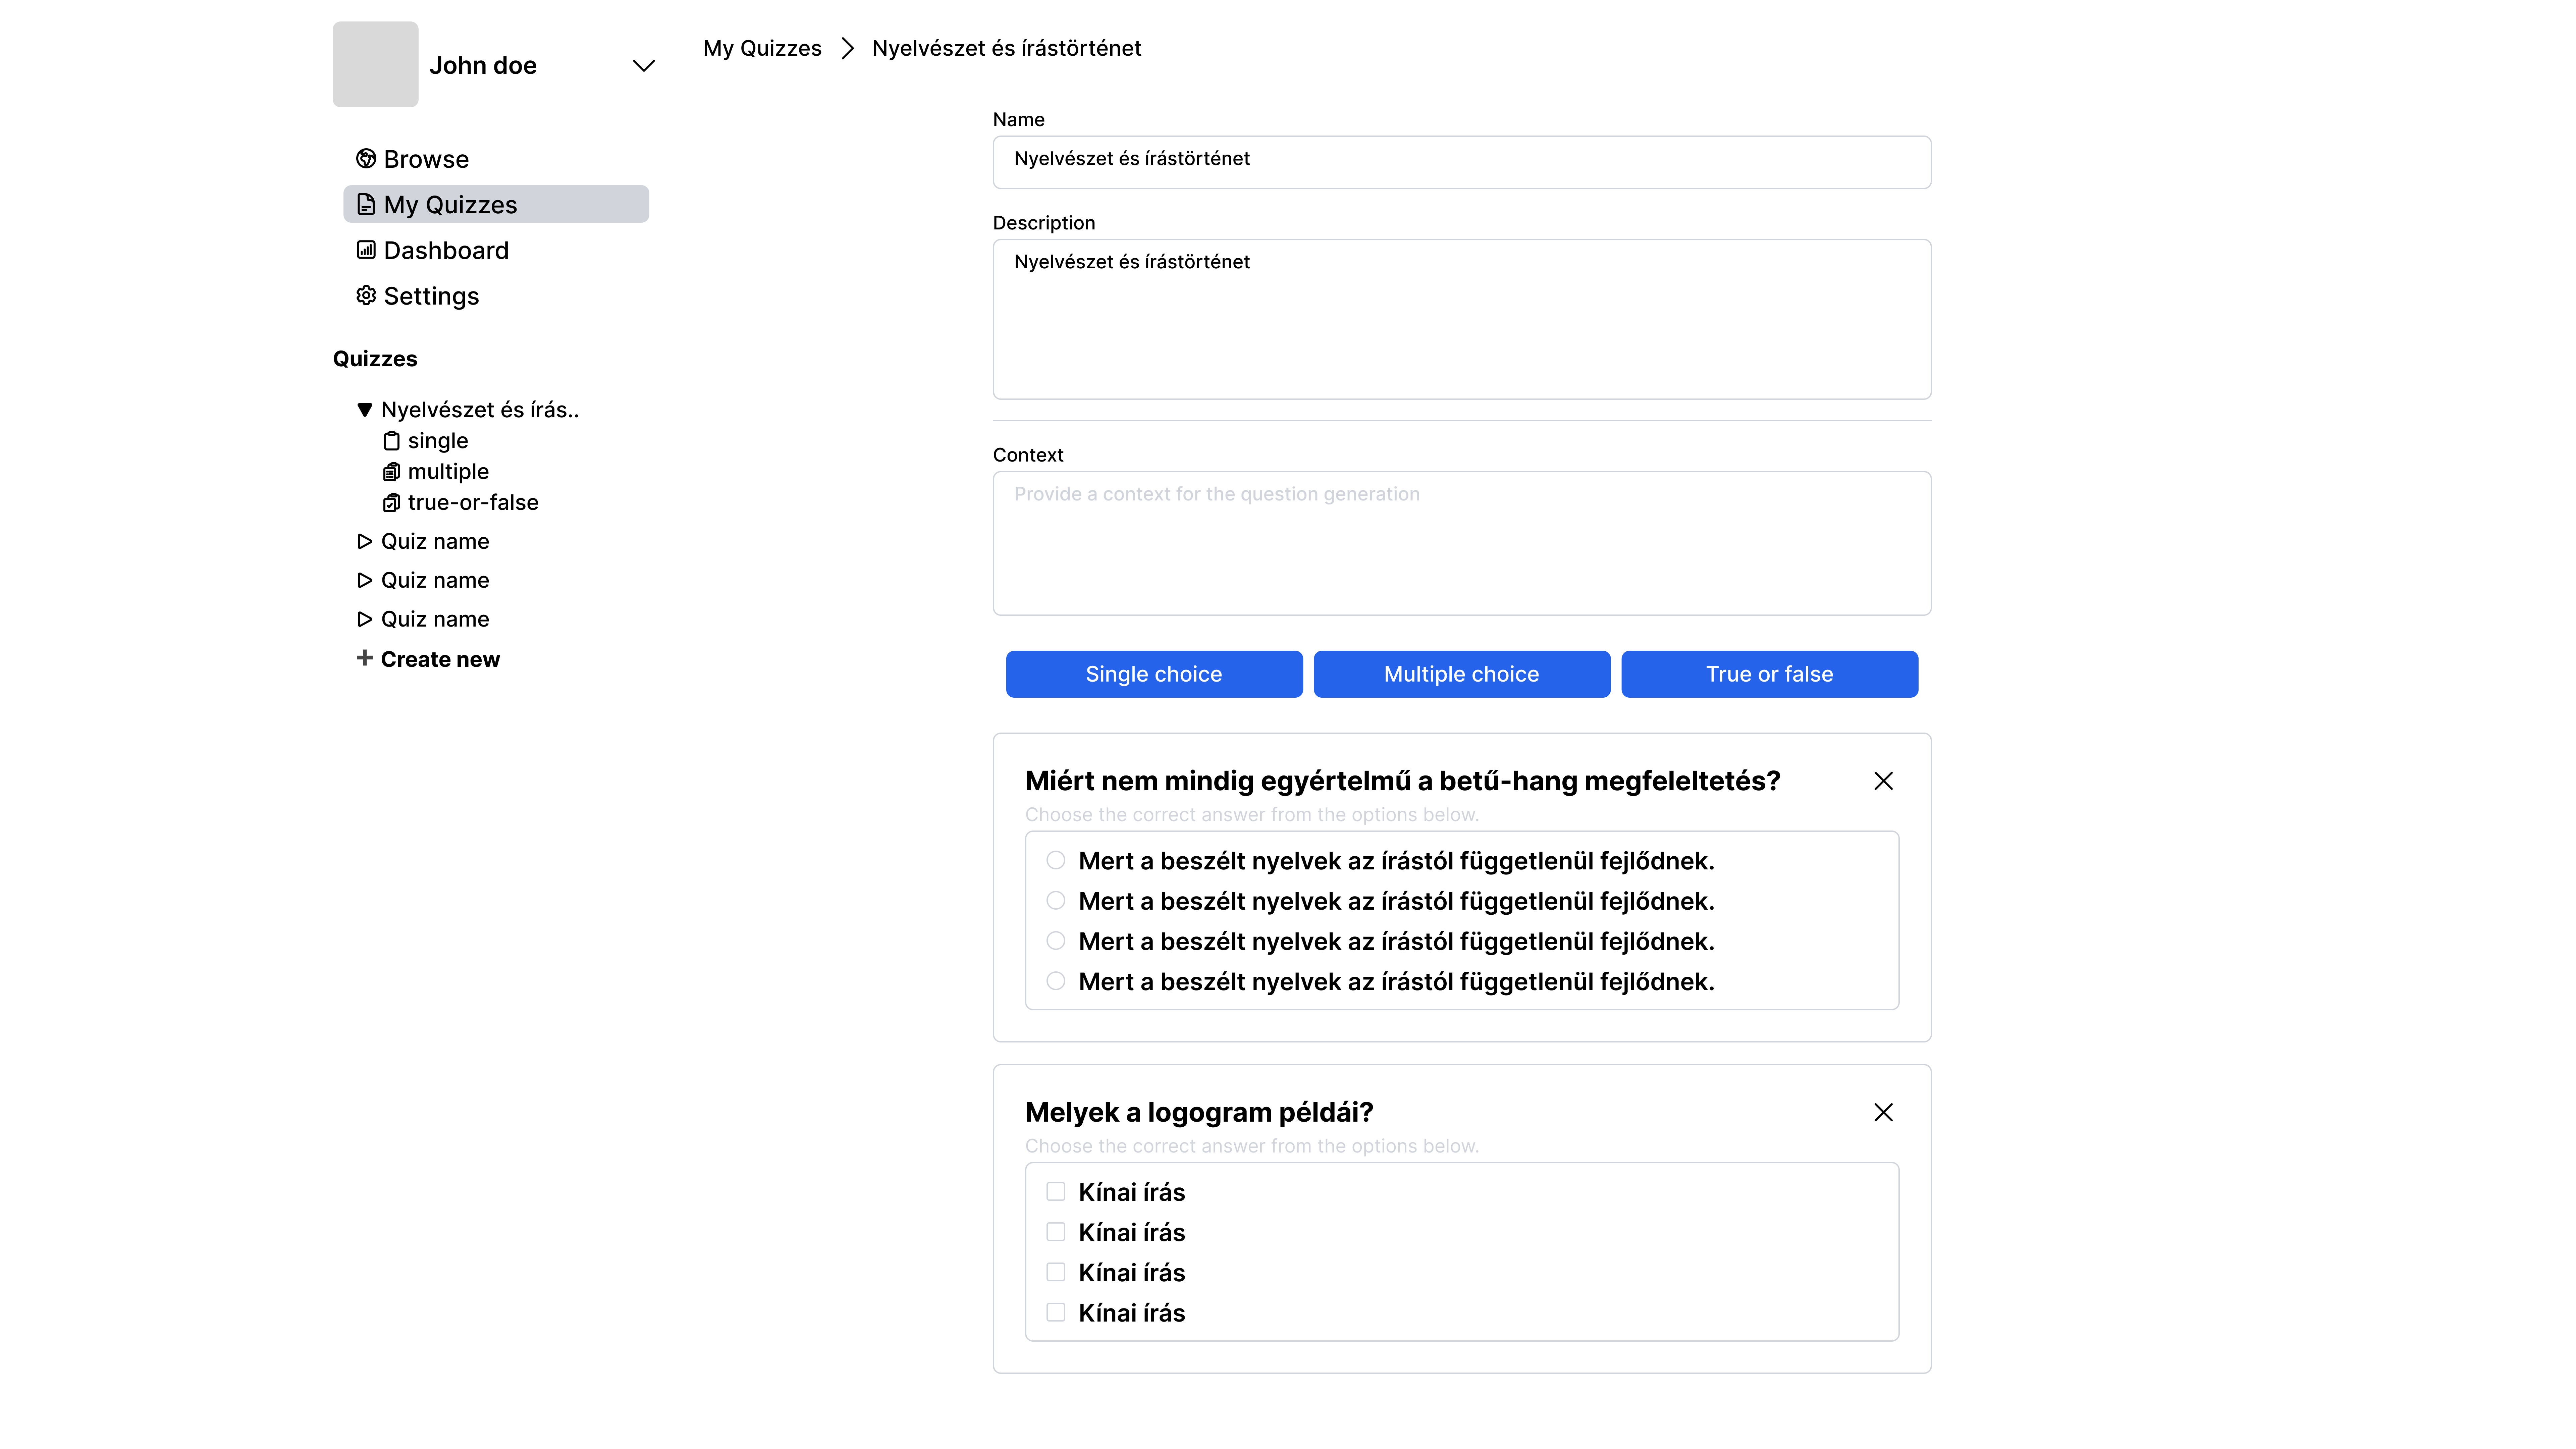
\includegraphics[width=0.8\textwidth, keepaspectratio]{figures/quiz-creation-page-initial-design.png}
    }
    \caption{Initial design of the creation page}
    \label{fig:quiz-creation-page-initial-design}
\end{figure}

I used the mockups as a starting point for the design because tailwindCSS allows fast prototyping. It turned out that implementing a not fully detailed design and changing the implementation is more rapid for me than creating a perfect design and implementing it later. It also allowed us to try out the concept in practice, thus preventing unnecessary iterations.

\subsubsection{User flow diagrams}

This subsection outlines the basic actions and navigations available through descriptions and diagrams. I have broken down the diagrams into smaller sections to make them easier to understand. 

The application's starting point for authenticated users is the \texttt{My Quizzes page}. After the login flow, the user can access some features directly or go to a different page. These functions and pages are described visually in this diagram~\ref{fig:flow-main}.

\begin{figure}[H]
    \centering
    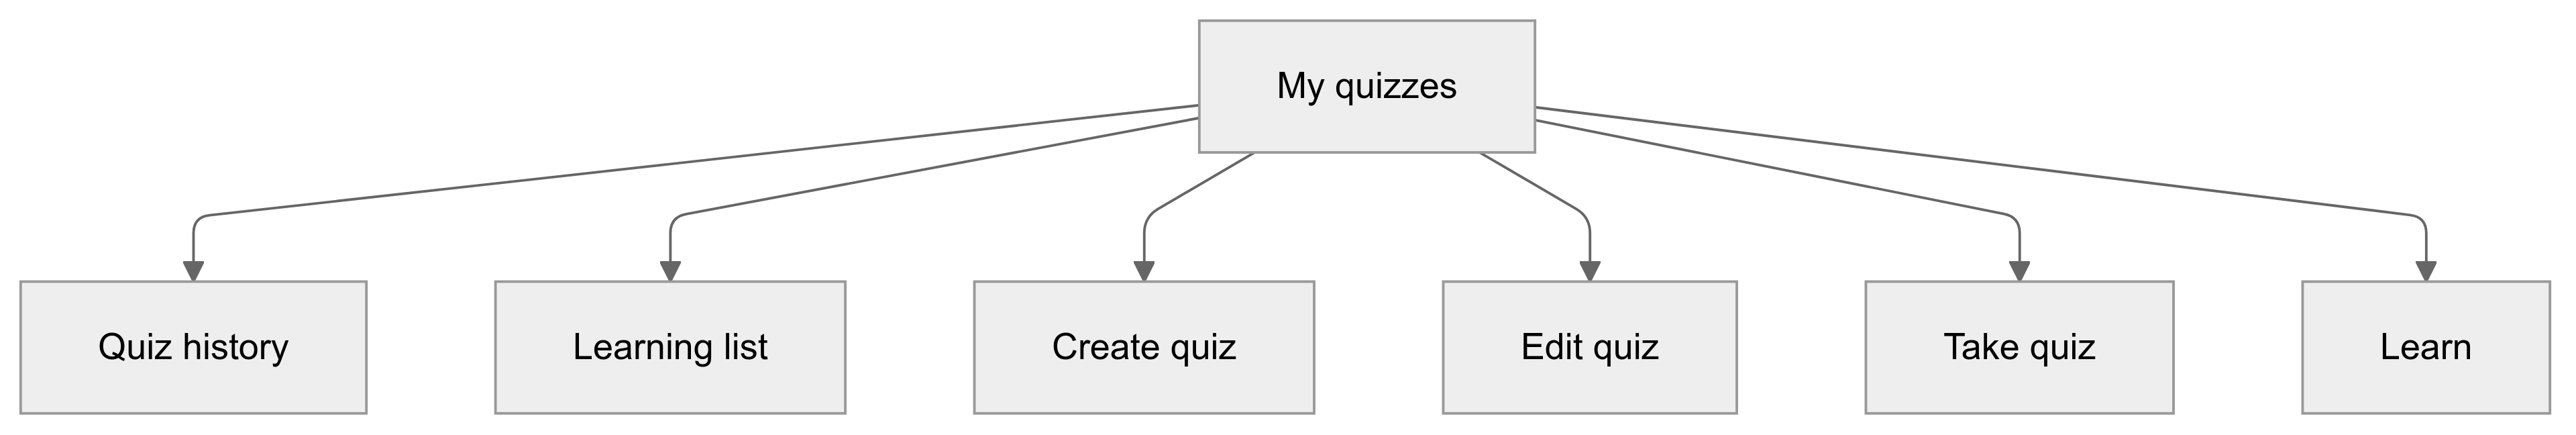
\includegraphics[width=0.8\textwidth, keepaspectratio]{figures/flow-main.png}
    \caption{Main navigation flow diagram}
    \label{fig:flow-main}
\end{figure}

The process of creating and editing a quiz is mostly identical. This flow is shown in figure~\ref{fig:flow-quiz-creation-and-edit}. The user can set the quiz title and description or provide a context for question generation. After that, the user can select a question type: single choice, multiple choice, or boolean, and the platform generates and shows the question using the context. Adding more questions or deleting already added ones are also available through this flow on this page.

\begin{figure}[H]
    \centering
    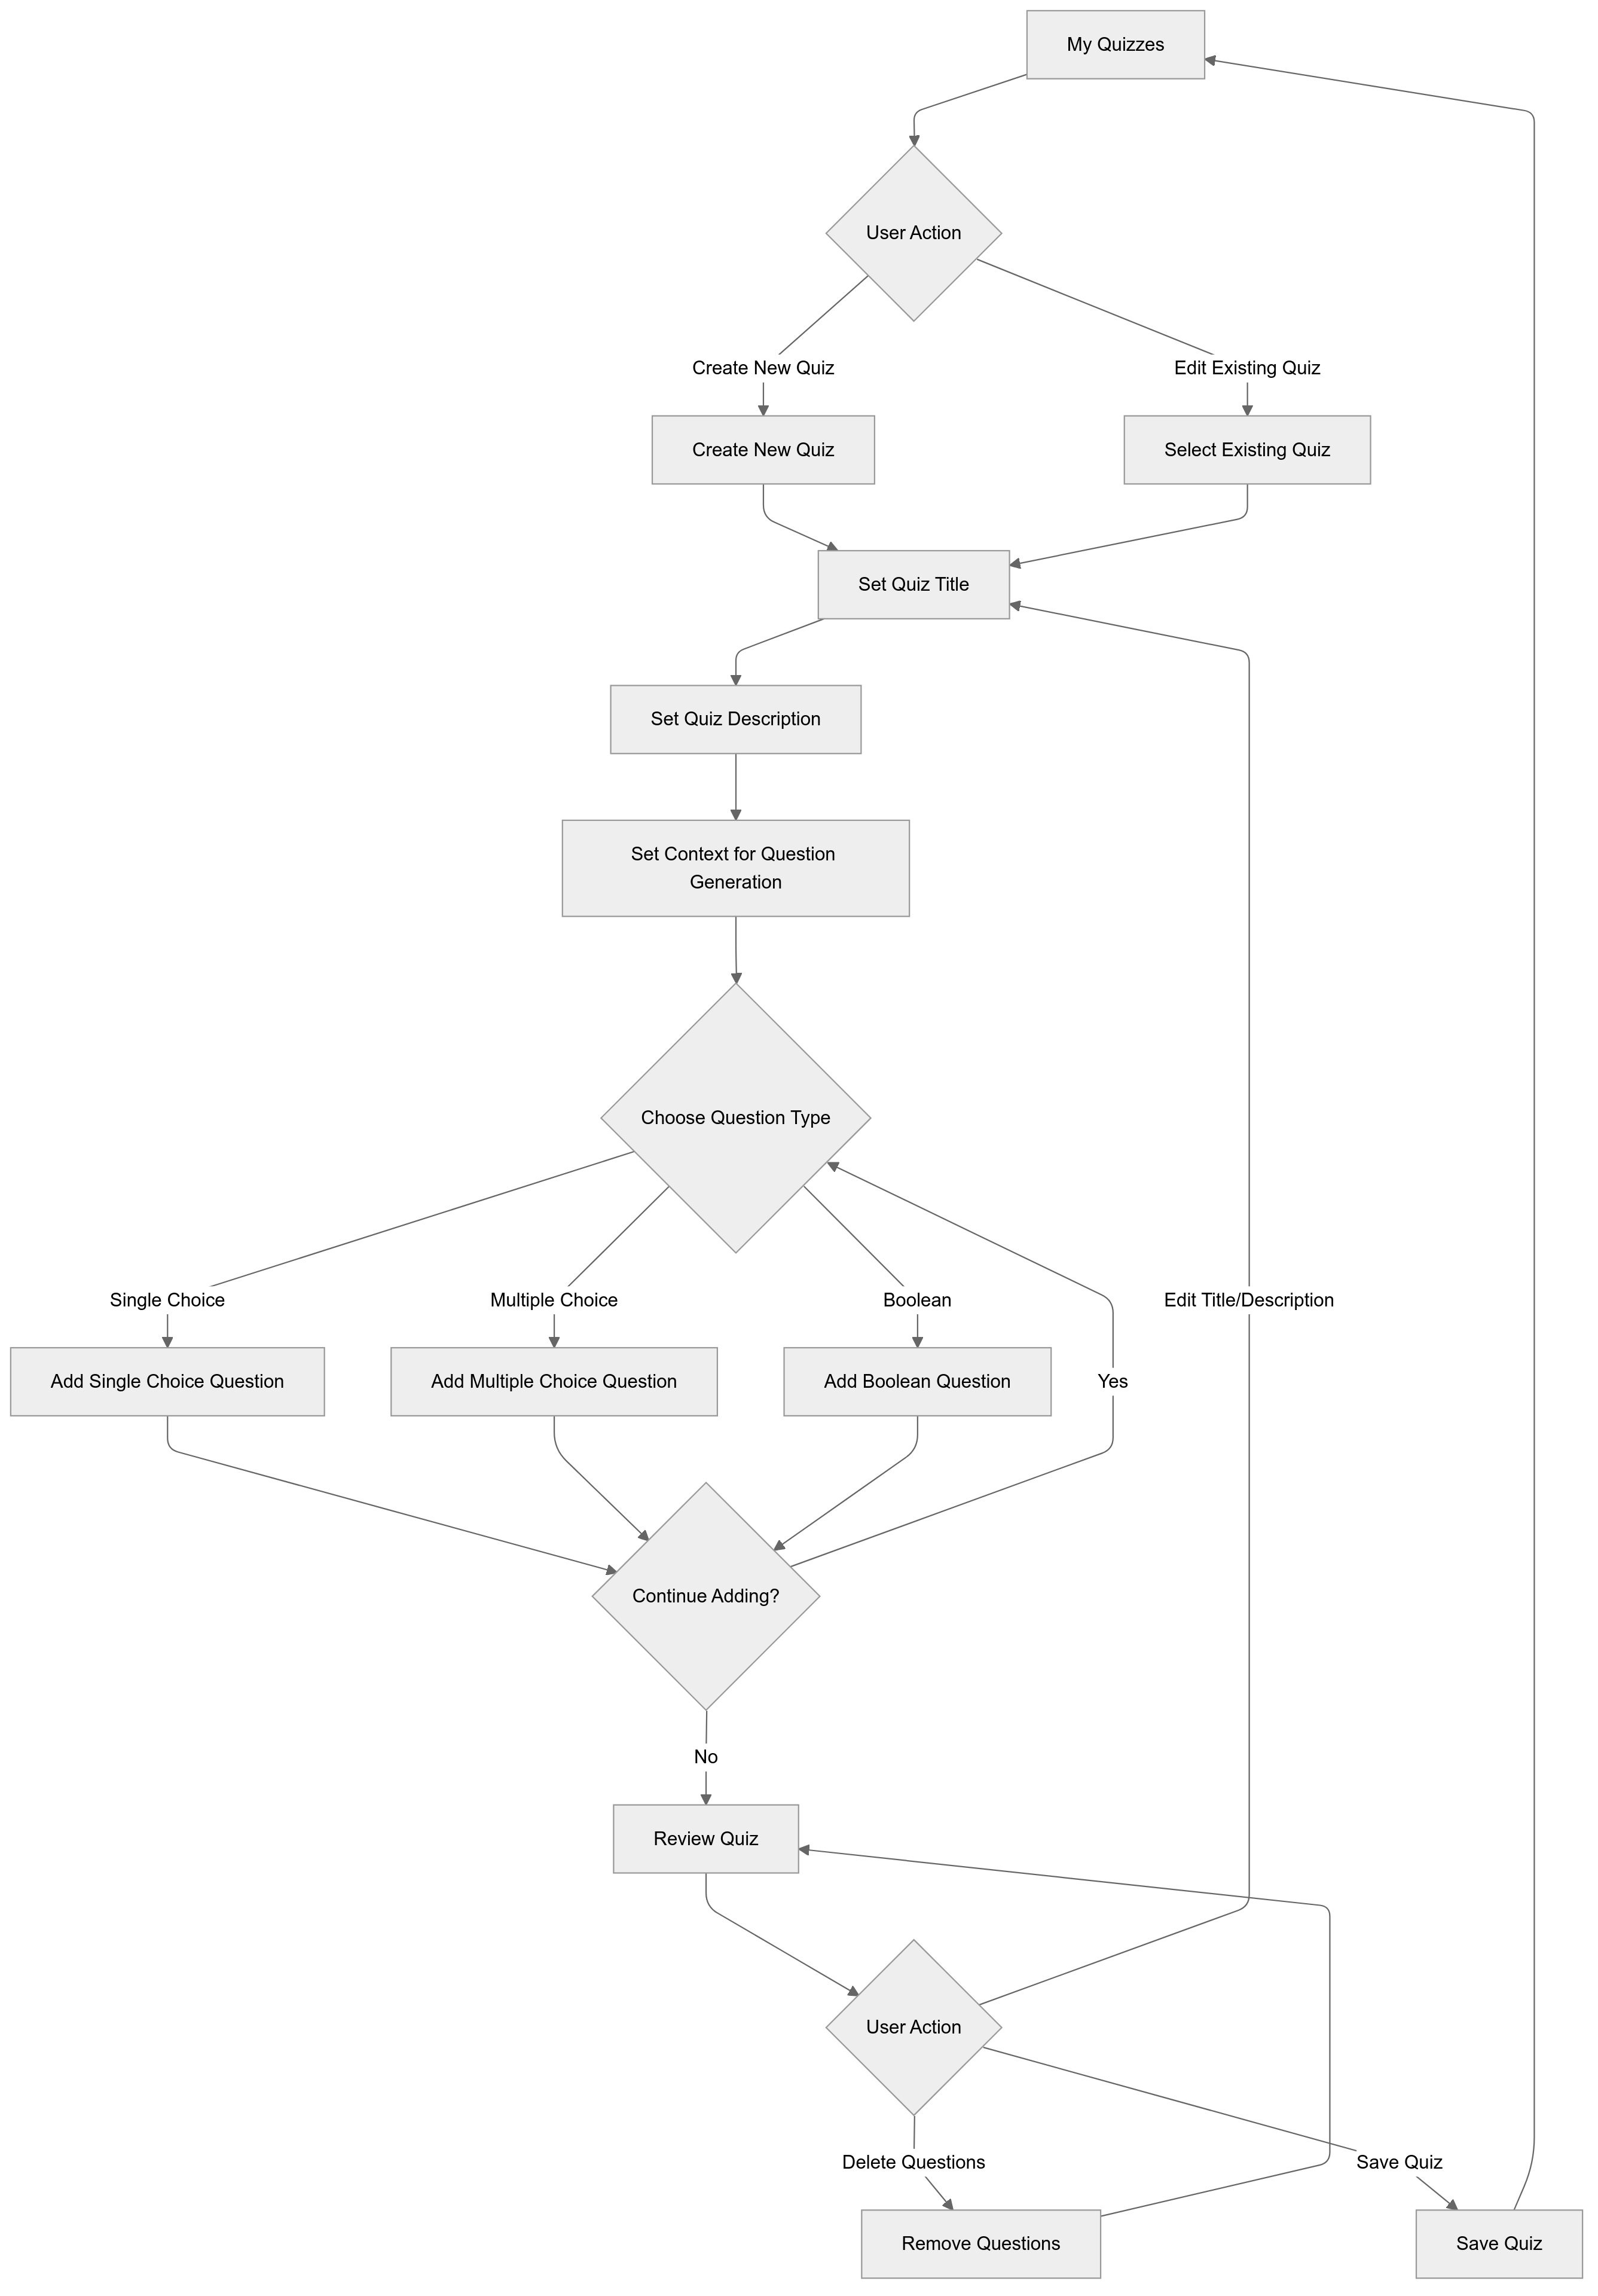
\includegraphics[width=0.9\textwidth, keepaspectratio]{figures/flow-quiz-creation-and-edit.png}
    \caption{Quiz creation and edit flow diagram}
    \label{fig:flow-quiz-creation-and-edit}
\end{figure}

When a user selects a quiz, the platform offers options to start taking it or continue an already-started but not finished one. When the user decides to start, a session is created, and the answers are saved automatically for this session. It stays open until the users submit their answers or start a new session. After closing, the user is redirected to the results, which can be viewed from the Quiz history page. This quiz-taking flow is also displayed in Figure~\ref{fig:flow-taking-quiz}.

\begin{figure}[H]
    \centering
    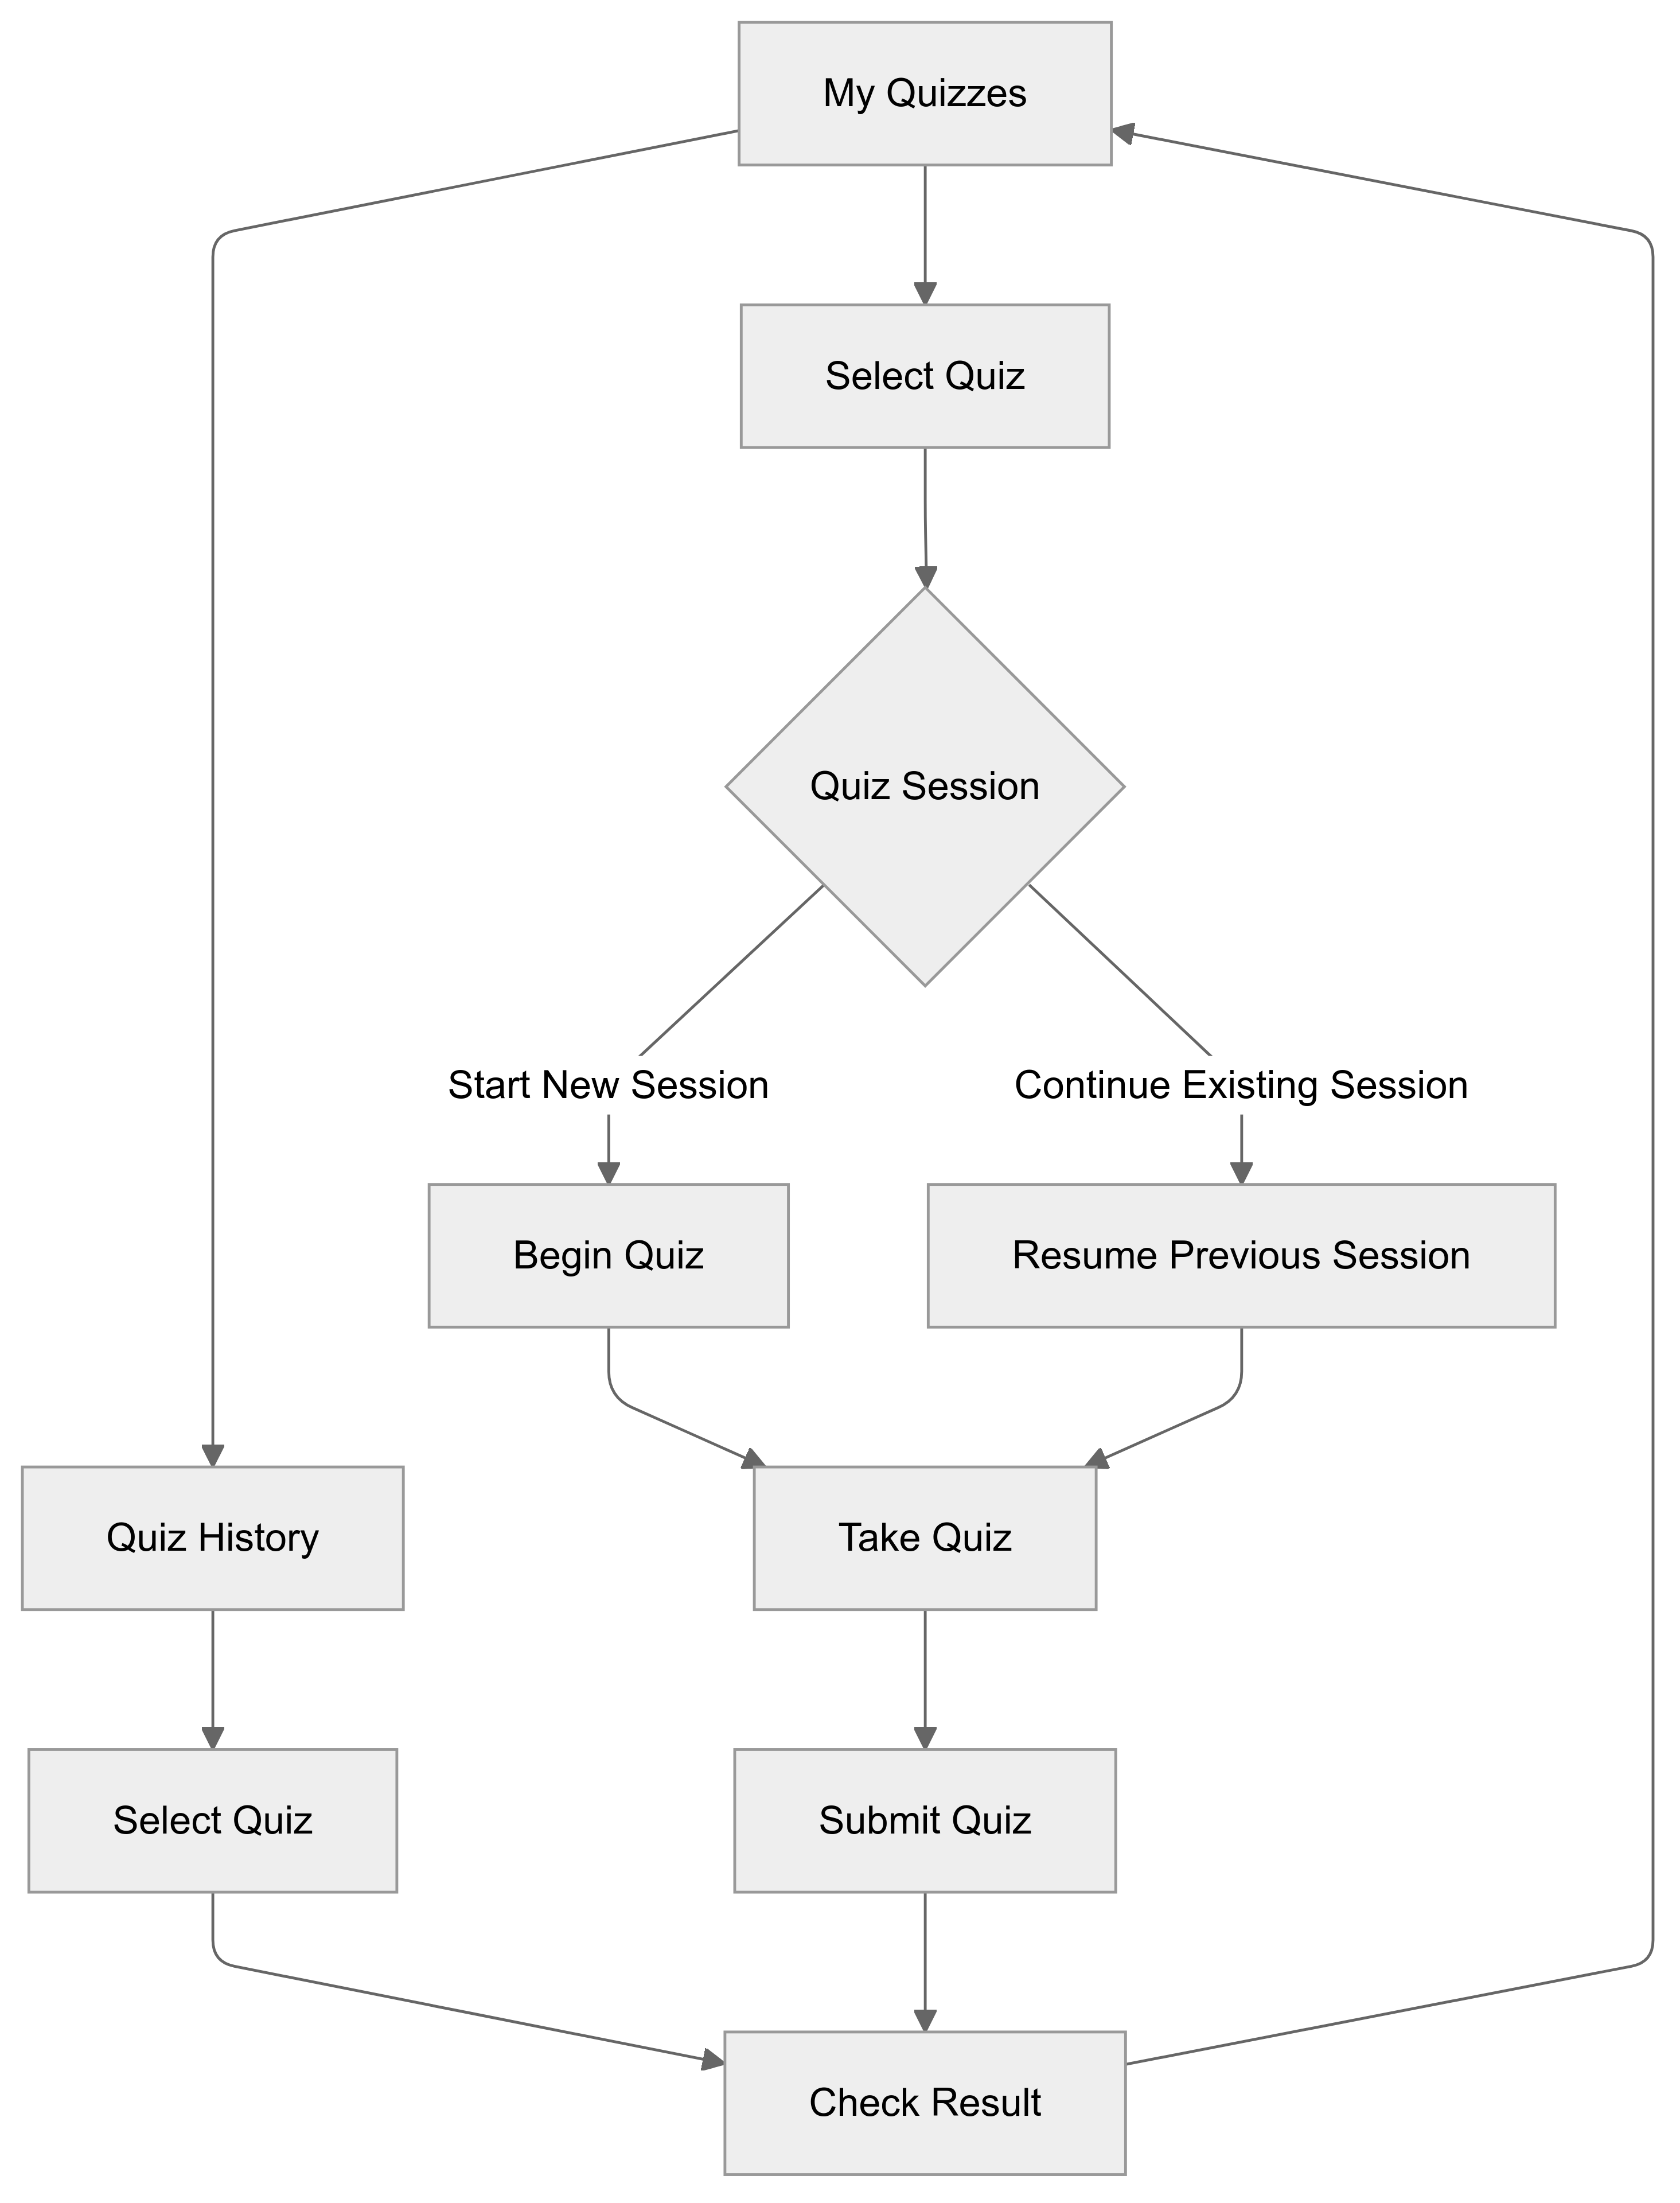
\includegraphics[width=0.8\textwidth, keepaspectratio]{figures/flow-taking-quiz.png}
    \caption{Taking quiz flow diagram}
    \label{fig:flow-taking-quiz}
\end{figure}

Reviewing questions is the core concept of spaced repetition. The users can manage which quizzes they want to learn, and the platform schedules them. The user can see and filter the questions scheduled for review on the Review page. It lists all the questions and adds options for the user to review. This review can be done one by one or simultaneously in the order specified by the platform. When the review is done, the platform schedules the questions for the following review and redirects the user to the learn page. Figure~\ref{fig:flow-review-item} displays this question reviewing flow.

\begin{figure}[H]
    \centering
    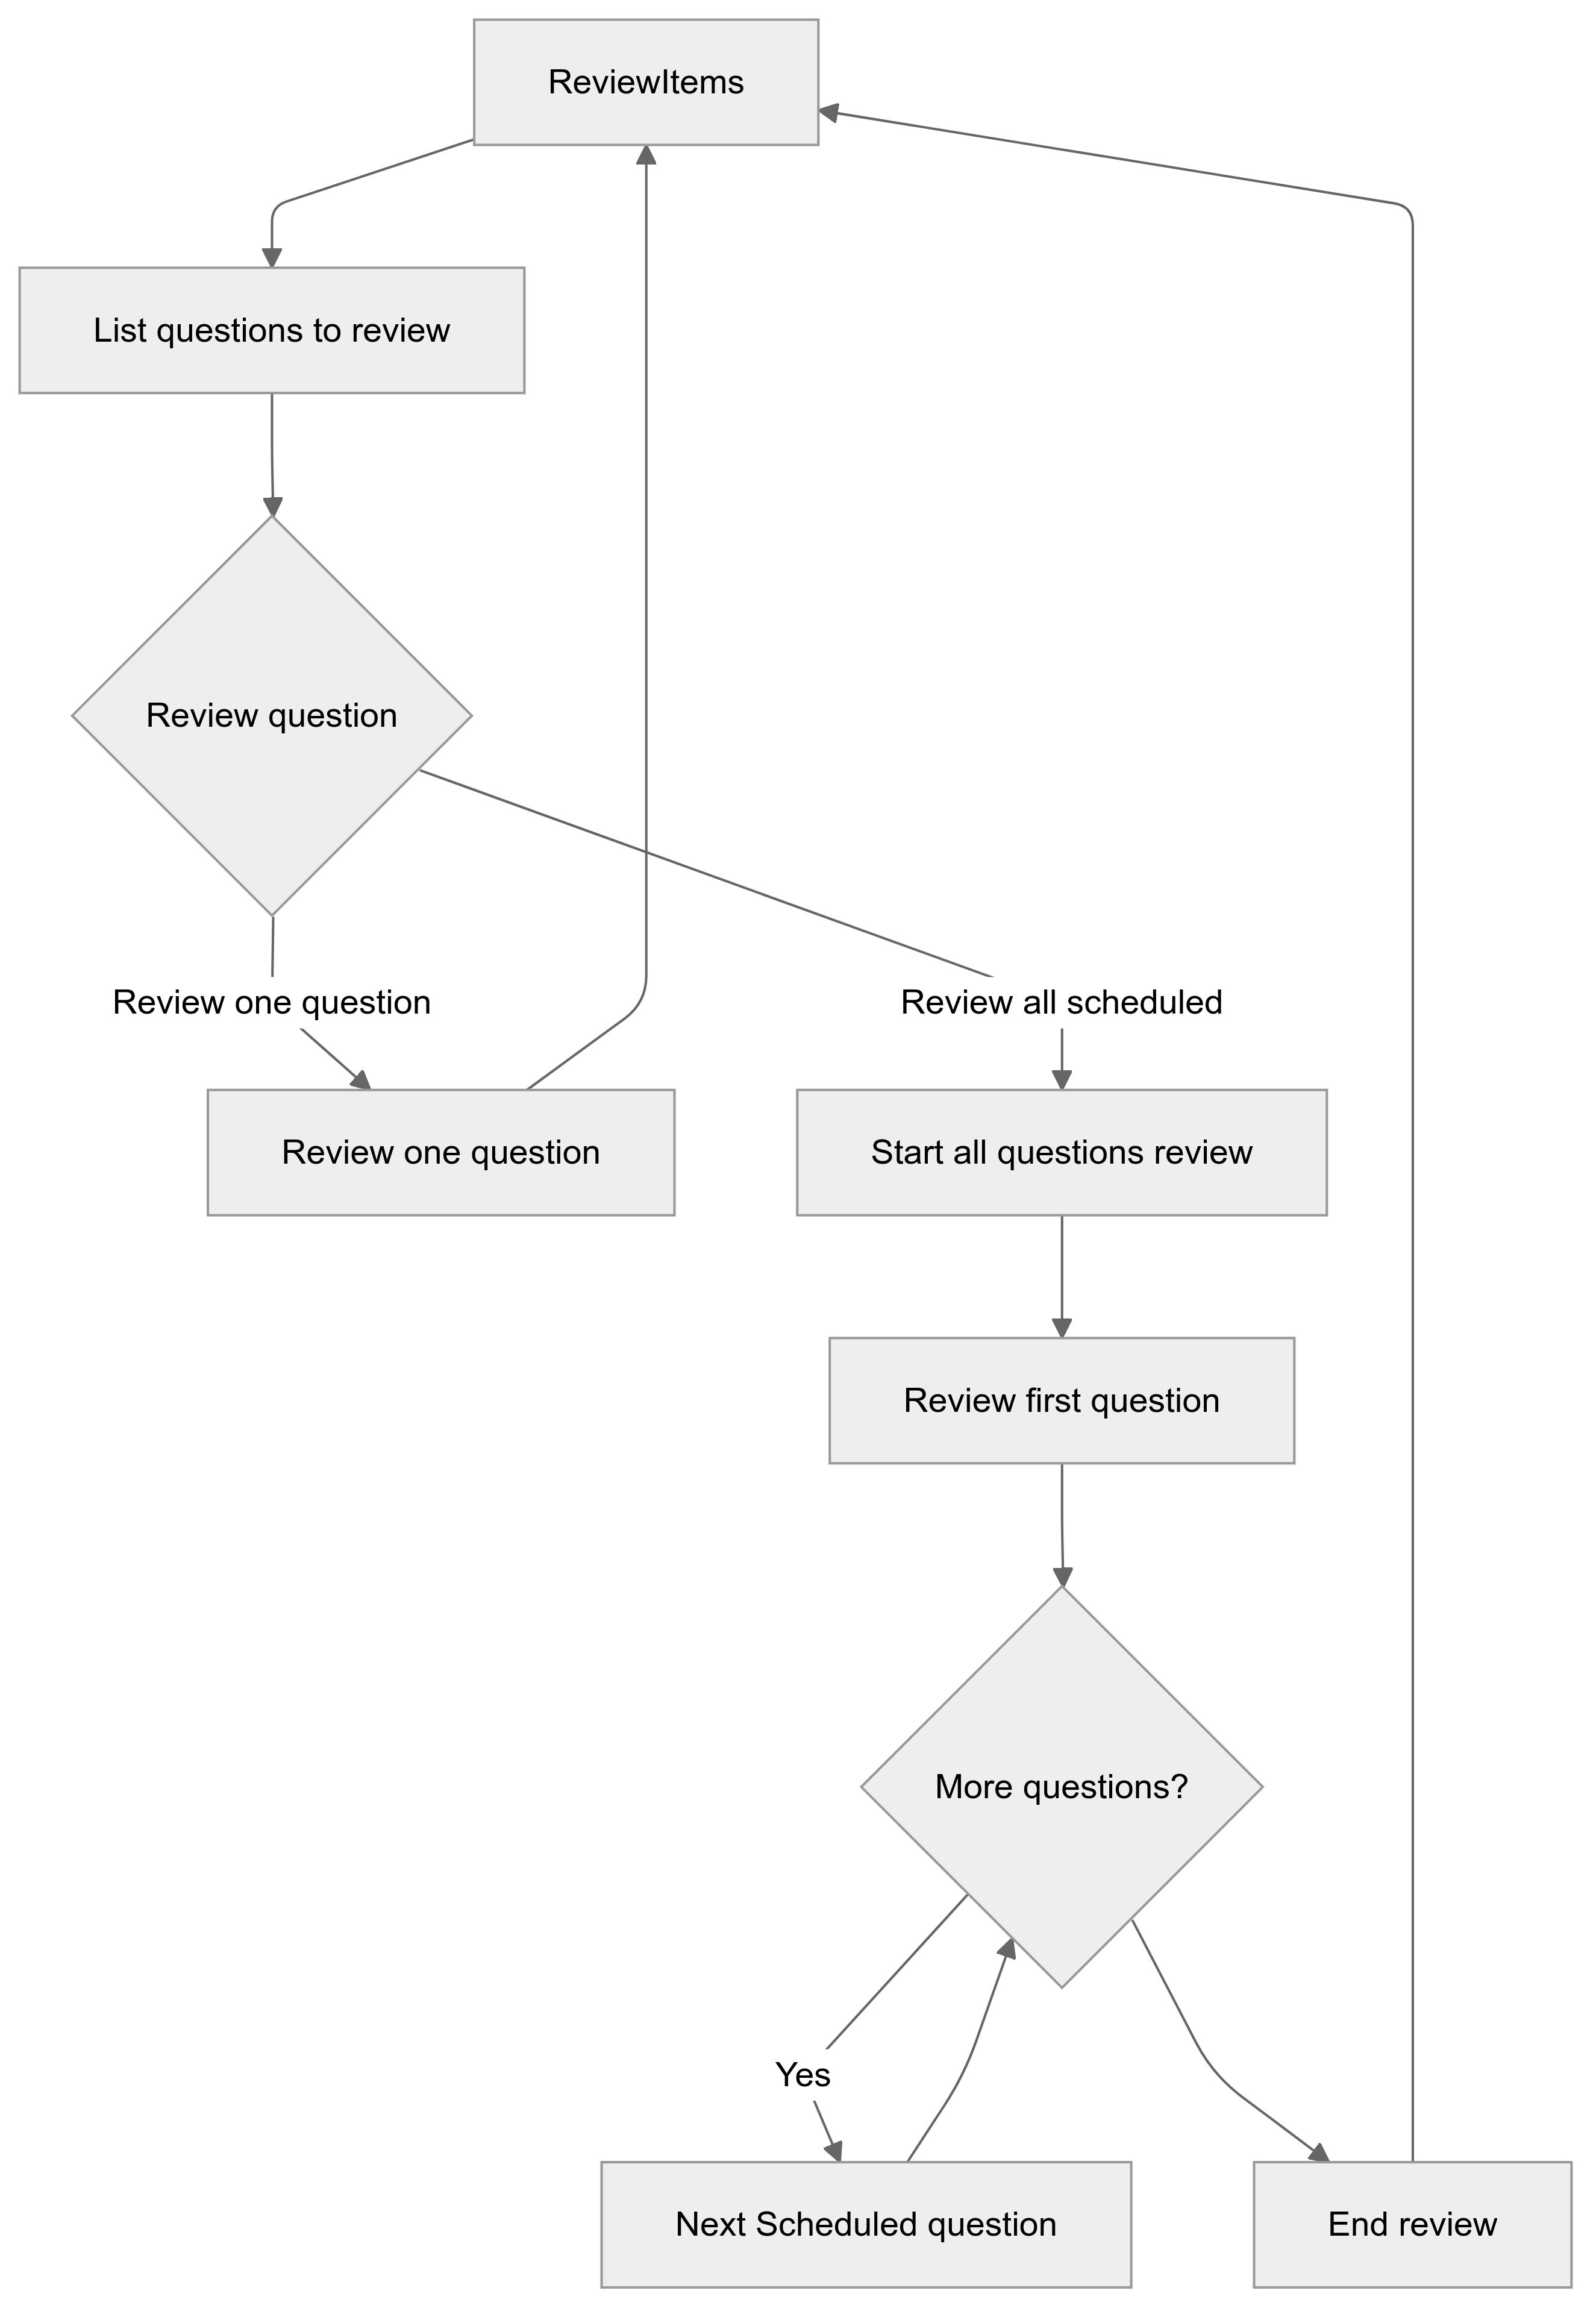
\includegraphics[width=0.8\textwidth, keepaspectratio]{figures/flow-review-item.png}
    \caption{Review items flow diagram}
    \label{fig:flow-review-item}
\end{figure}

\section{Backend Design}

The backend service is a monolith-styled web service. It is a traditional API server that accesses the platform's functionalities. It is responsible for input validation, business logic, and data access and integrates external services like the question generator LLM. Overall, it is the core of the platform that acts as a glue service. This section outlines the backend service's architecture at a higher level, presents the main business logic and patterns used, and covers security.

\subsection{High-level architecture}

This service uses a generic three-layered architecture (presentation, business, and data access layers) but does not follow a specific architectural pattern like MVC. Figure~\ref{fig:backend-architecture} shows these layers and their relations.

\begin{figure}[H]
    \centering
    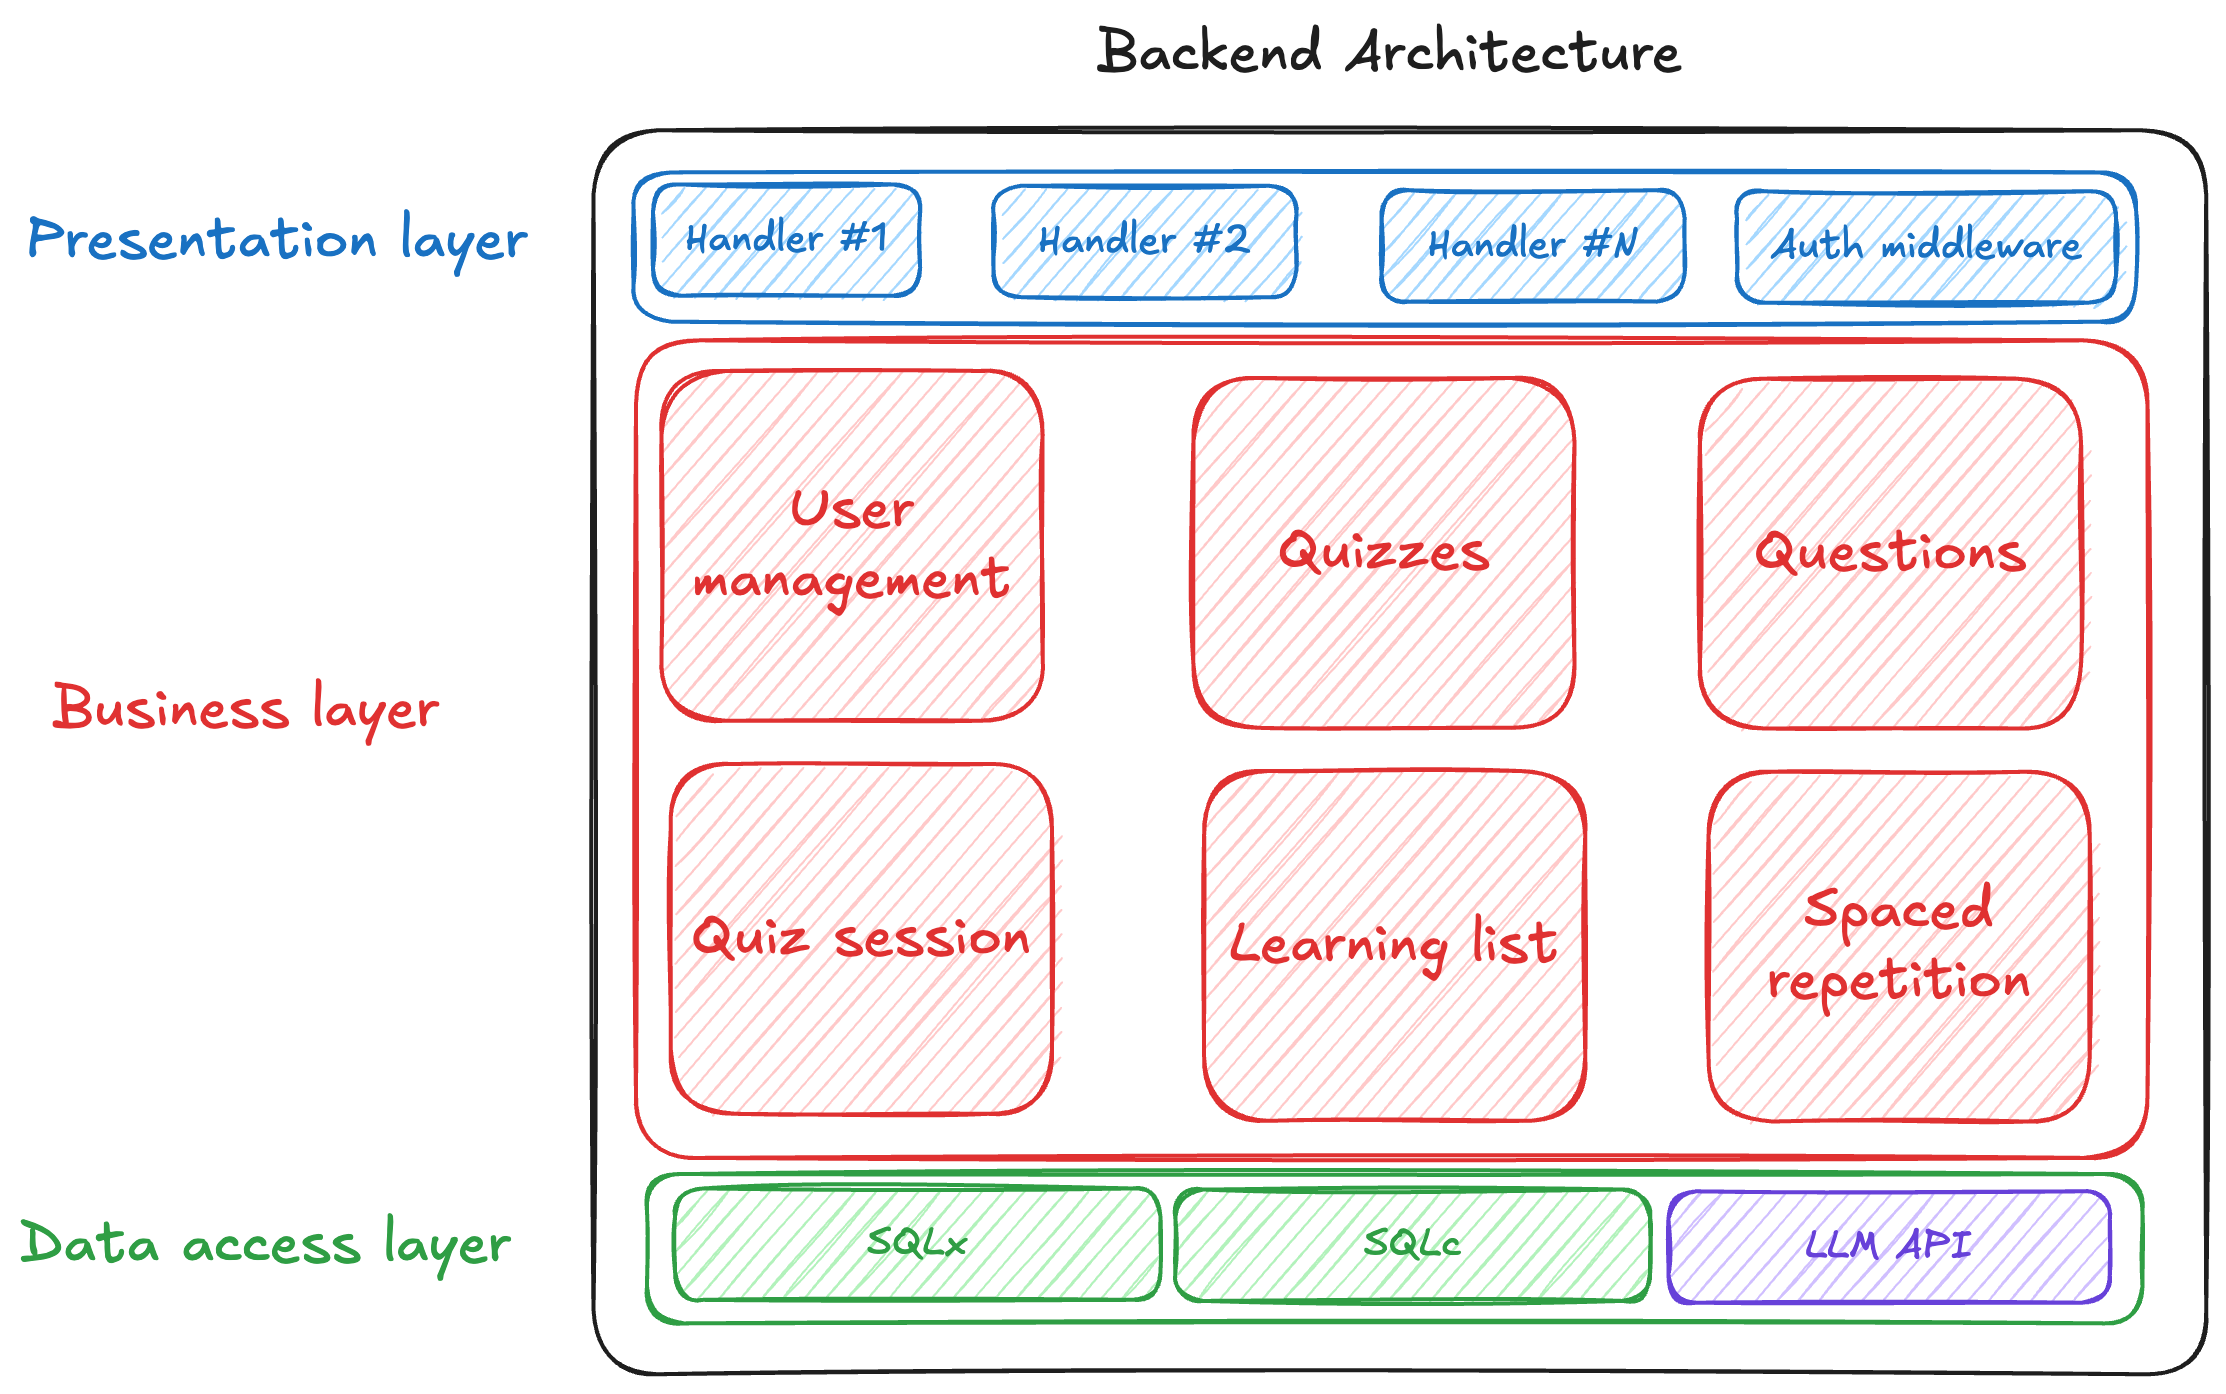
\includegraphics[width=0.8\textwidth, keepaspectratio]{figures/backend-architecture.png}
    \caption{Review items flow diagram}
    \label{fig:backend-architecture}
\end{figure}

The presentation layer handles the requests from the client-server and creates the JSON responses. This thin layer on top of the architecture ensures access to outside services. It is also responsible for validating and sanitizing user input. The authentication and error handling middleware are lying in this layer.

The business logic layer contains almost everything for the platform. All the features are found here. It is between the presentation and data access layers (DAL). Components from this layer process the validated requests, retrieve data from external sources relying on the DAL, and do the platform's business logic. By separating the functions logically, these components can be named User management, Quizzes, Questions, Quiz sessions, Learning list, and Spaced repetition.

The data access layer is a thin layer that abstracts data retrieved from different sources. The platform gets data from the database through the two SQL libraries (SQLx and SQLc) and the AI service through its REST interface by HTTP request. It is responsible for parsing and mapping the data into a processable format for the upper layers.

\subsection{API design}

The API design follows a traditional REST approach using JSON requests and responses. This design respects the different HTTP methods used for their purposes. The endpoints do not use any versioning system because this is the first version of the service and has yet to undergo any significant redesign. Later, introducing versioning can be beneficial, but it is not necessary now.

\subsubsection{API Categories}

API endpoints are categorized into two leading groups: those available for the user without authentication and those that require authentication. The unauthenticated endpoints are only for signing up for a new user account or logging into an existing account. The other group is categorized into a few smaller categories based on functionality.

\textbf{Quizzes} The endpoints in this category relate to managing quizzes. This endpoint allows for creating new quizzes and modifying or deleting existing ones.

\textbf{Questions} The question-related endpoints are for generating questions with the AI services using the given user context. These are also for managing the questions linked to quizzes.

\textbf{Quiz sessions} The quiz session endpoints are for creating a session when the user decides to take a quiz and storing the answers. It also closes the sessions when needed and manages the quiz results.

\textbf{Learning list} These endpoints allow the user to add quizzes to its learning list or remove them from it. They also trigger scheduling when a user adds a new quiz to its list.

\textbf{Review items} These are the endpoints for listing the scheduled questions to review by the spaced repetition algorithm. They handle the review process by offering the questions and calculating the upcoming schedules.

\subsubsection{Request and response patterns}

The backend service communicates with the backend with standard HTTP messages. While the clients expect the data to be in form-data format or url-encoded-form-data, it does it in JSON. Figure~\ref{lst:http-request-and-response} shows an example request and its response processed by the server in HTTP format.

\begin{lstlisting}[caption=HTTP request and response for authentication,label=lst:http-request-and-response]
---- Authentication request:

POST /authenticate-user HTTP/1.1
Host: localhost:9000
Content-Type: application/json
Content-Length: 68

{ "email": "john.doe@email.com", "password": "password123" }

---- Authentication response:

HTTP/1.1 200 OK
Content-Type: application/json; charset=UTF-8
Set-Cookie: session=93f4b04b-9df0-49c2-8c04-794ffdb63526; Expires=Sat, 30 Nov 2024 17:25:37 GMT; HttpOnly
Date: Sat, 30 Nov 2024 16:26:37 GMT
Content-Length: 93

{"id":"7c9ea74d-6078-4338-b5ee-7a788f8a57ca","name":"John Doe","email":"john.doe@email.com"}
\end{lstlisting}

\subsubsection{Error-handling patterns}

The Go language has an explicit error-handling mechanism; it forces the developer to handle the error. When a developer follows these rules correctly, a nice structure of error messages can be built. This message is usually good for logging and informing the caller what problem happened during the request's serving. Also, Echo supports wrapping the Go errors into HTTP error messages with error codes, which can be a convenient and consistent form of error handling. Listing~\ref{lst:error-handling-pattern} shows an example of calling a service; when it runs on an error, use its message as a response.

\begin{lstlisting}[caption=Error handling using Go errors,label=lst:error-handling-pattern]
// Calculate score for the given review item
score, err := calculateReviewItemScore(reviewItem, answers)
if err != nil {
    return echo.NewHTTPError(http.StatusInternalServerError, fmt.Errorf("calculating score for review item with ID %q: %w\n", reviewItemID, err))
}
\end{lstlisting}

\subsubsection{Endpoint overview}

The API design is created using Postman\footnote{https://www.postman.com/}.The following tables list the application's endpoints grouped by categories.

% auth
\begin{table}[H]
    \begin{tabular}{|l|l|l|}
        \hline
        \textbf{URL} & \textbf{Method} & \textbf{Description} \\
        \hline
        /authenticate-user & POST & Authenticate the user \\
        /authenticated & GET & Check authentication \\
        /create-user & POST & Create a user \\
        /delete-user/:id & DELETE & Delete a user \\
        /logout & POST & Logout the user \\
        \hline
    \end{tabular}
    \caption{Auth endpoint overview}
    \label{tab:auth-endpoints}
\end{table}

% quizzes
\begin{table}[H]
    \begin{tabular}{|l|l|l|}
        \hline
        \textbf{URL} & \textbf{Method} & \textbf{Description} \\
        \hline
        /quizzes/:id & GET & Get a quiz \\
        /quizzes/:id & PATCH & Update a quiz \\
        /quizzes/:id & DELETE & Delete a quiz \\
        /quizzes/user/:id & GET & Get the user's quizzes \\
        /quizzes/create & POST & Create a quiz \\
        \hline
    \end{tabular}
    \caption{Quiz endpoint overview}
    \label{tab:quiz-endpoints}
\end{table}

% question
\begin{table}[H]
    \begin{tabular}{|c|p{5cm}|l|p{5.5cm}|}
        \hline
        \textbf{Question type} & \textbf{URL} & \textbf{Method} & \textbf{Description} \\
        \hline
        Single choice & /questions/single-choice & POST & Generate a single choice question \\
        & /questions/single-choice/:id & GET & Get a single choice question \\
        & /questions/single-choice/:id & PATCH & Update a single choice question \\
        & /questions/single-choice/:quizId/:id & DELETE & Delete a single choice question \\
        \hline
        Multiple choice & /questions/multiple-choice & POST & Generate a multiple choice question \\
        & /questions/multiple-choice/:id & GET & Get a multiple choice question \\
        & /questions/multiple-choice/:id & PATCH & Update a multiple choice question \\
        & /questions/multiple-choice/:quizId/:id & DELETE & Delete a multiple choice question \\
        \hline
        Boolean & /questions/true-or-false & POST & Generate a boolean choice question \\
        & /questions/true-or-false/:id & GET & Get a boolean choice question \\
        & /questions/true-or-false/:id & PATCH & Update a boolean choice question \\
        & /questions/true-or-false/:quizId/:id & DELETE & Delete a boolean choice question \\
        \hline
    \end{tabular}
    \caption{Question endpoint overview}
    \label{tab:question-endpoints}
\end{table}

% quiz sessions
\begin{table}[H]
    \begin{tabular}{|l|l|l|}
        \hline
        \textbf{URL} & \textbf{Method} & \textbf{Description} \\
        \hline
        /quiz-sessions/:quizSessionId & GET & Get a quiz session \\
        /quiz-sessions/ & GET & Get quiz sessions \\
        /quiz-sessions/has-open & GET & Check has an open quiz session \\
        /quiz-sessions/start & POST & Start a quiz session \\
        /quiz-sessions/:quizSessionId/submit & POST & Submit quiz and finish its session \\
        /quiz-sessions/:quizSessionId/result & GET & Get quiz result \\
        /quiz-sessions/:quizSessionId/answers & GET & Get quiz session answers \\
        /quiz-sessions/:quizSessionId/answers & PUT & Update a quiz session answer \\
        \hline
    \end{tabular}
    \caption{Quiz session endpoint overview}
    \label{tab:quiz-session-endpoints}
\end{table}

% quiz history and learn list
\begin{table}[H]
    \begin{tabular}{|l|l|l|}
        \hline
        \textbf{URL} & \textbf{Method} & \textbf{Description} \\
        \hline
        /quiz-history & GET & Get quiz history entries \\
        /learn-list & GET & Get learning list \\
        /learn-list/:quizID/add & POST & Add quiz to learning list \\
        /learn-list/:quizID/remove & POST & Remove quiz from learning list \\
        \hline
    \end{tabular}
    \caption{Quiz history endpoint overview}
    \label{tab:quiz-history-endpoints}
\end{table}

% review items
\begin{table}[H]
    \begin{tabular}{|l|l|p{5.5cm}|}
        \hline
        \textbf{URL} & \textbf{Method} & \textbf{Description} \\
        \hline
        /review-items & GET & Get review items \\
        /review-items/quiz-options & GET & Get quiz options \\
        /review-items/item-counts & GET & Count scheduled and unscheduled questions \\
        /review-items/get-question/:reviewItemID & GET & Get review item question \\
        /review-items/get-question & GET & Get question \\
        /review-items/:reviewItemID/submit & POST & Submit review item question \\
        \hline
    \end{tabular}
    \caption{Review item endpoint overview}
    \label{tab:review-items-endpoints}
\end{table}

\subsection{Security}

Security is one of an application's critical aspects. Nowadays, these security features in software not only protect users and platform assets but are also part of the user experience. Without them, no application would exist. Achieving properly secure applications is not easy and is more than just a one-off task because it requires periodic review.

\subsubsection{Authentication}

Authentication is the process of identifying the user who has accessed software. There are several ways to do it:

\begin{itemize}
    \item \textbf{User credential-based authentication}: This authenticates the user through identifiers and pre-shared secrets such as passwords. This way is not recommended today because it requires repeatedly sharing the secret, making it easier to eavesdrop.
    \item \textbf{Session-based authentication}: In this way, a session is created on the server after authentication with credentials. A session ID is also issued by the server for the user for later authentications. This session stores the state on the server and, usually, has an expiry and can be explicitly destroyed if necessary.
    \item \textbf{Token-based authentication}: Token-based authentication is similar to session-based authentication, but in this case, the state is stored in a token on the client. The server issues and signs these tokens after successful user authentication. The client sends the token to the server for authentication and authorization purposes. One of its downfalls is that it is hard to invalidate these tokens, requiring complex token management solutions.
    \item \textbf{Other forms}: There are numerous more ways to do it, like OAuth (with many extensions), but for the platform, We chose a more uncomplicated solution, so I  do not detail them now.
\end{itemize}

We chose a session cookie-based form for the platform, which felt simple yet powerful for our use case. Session-based solutions suit us better for the monolith architecture because the state can be stored in a single server and does not have to be synchronized by other instances. The server issues the session token as HTTP cookies and sends it to the client after the user completes the login flow. The authentication-requiring endpoints check that this cookie exists and is valid before continuing to process the requests. Figure~\ref{fig:authentication-sequence} shows the login flow with session cookies.

\begin{figure}[H]
    \centering
    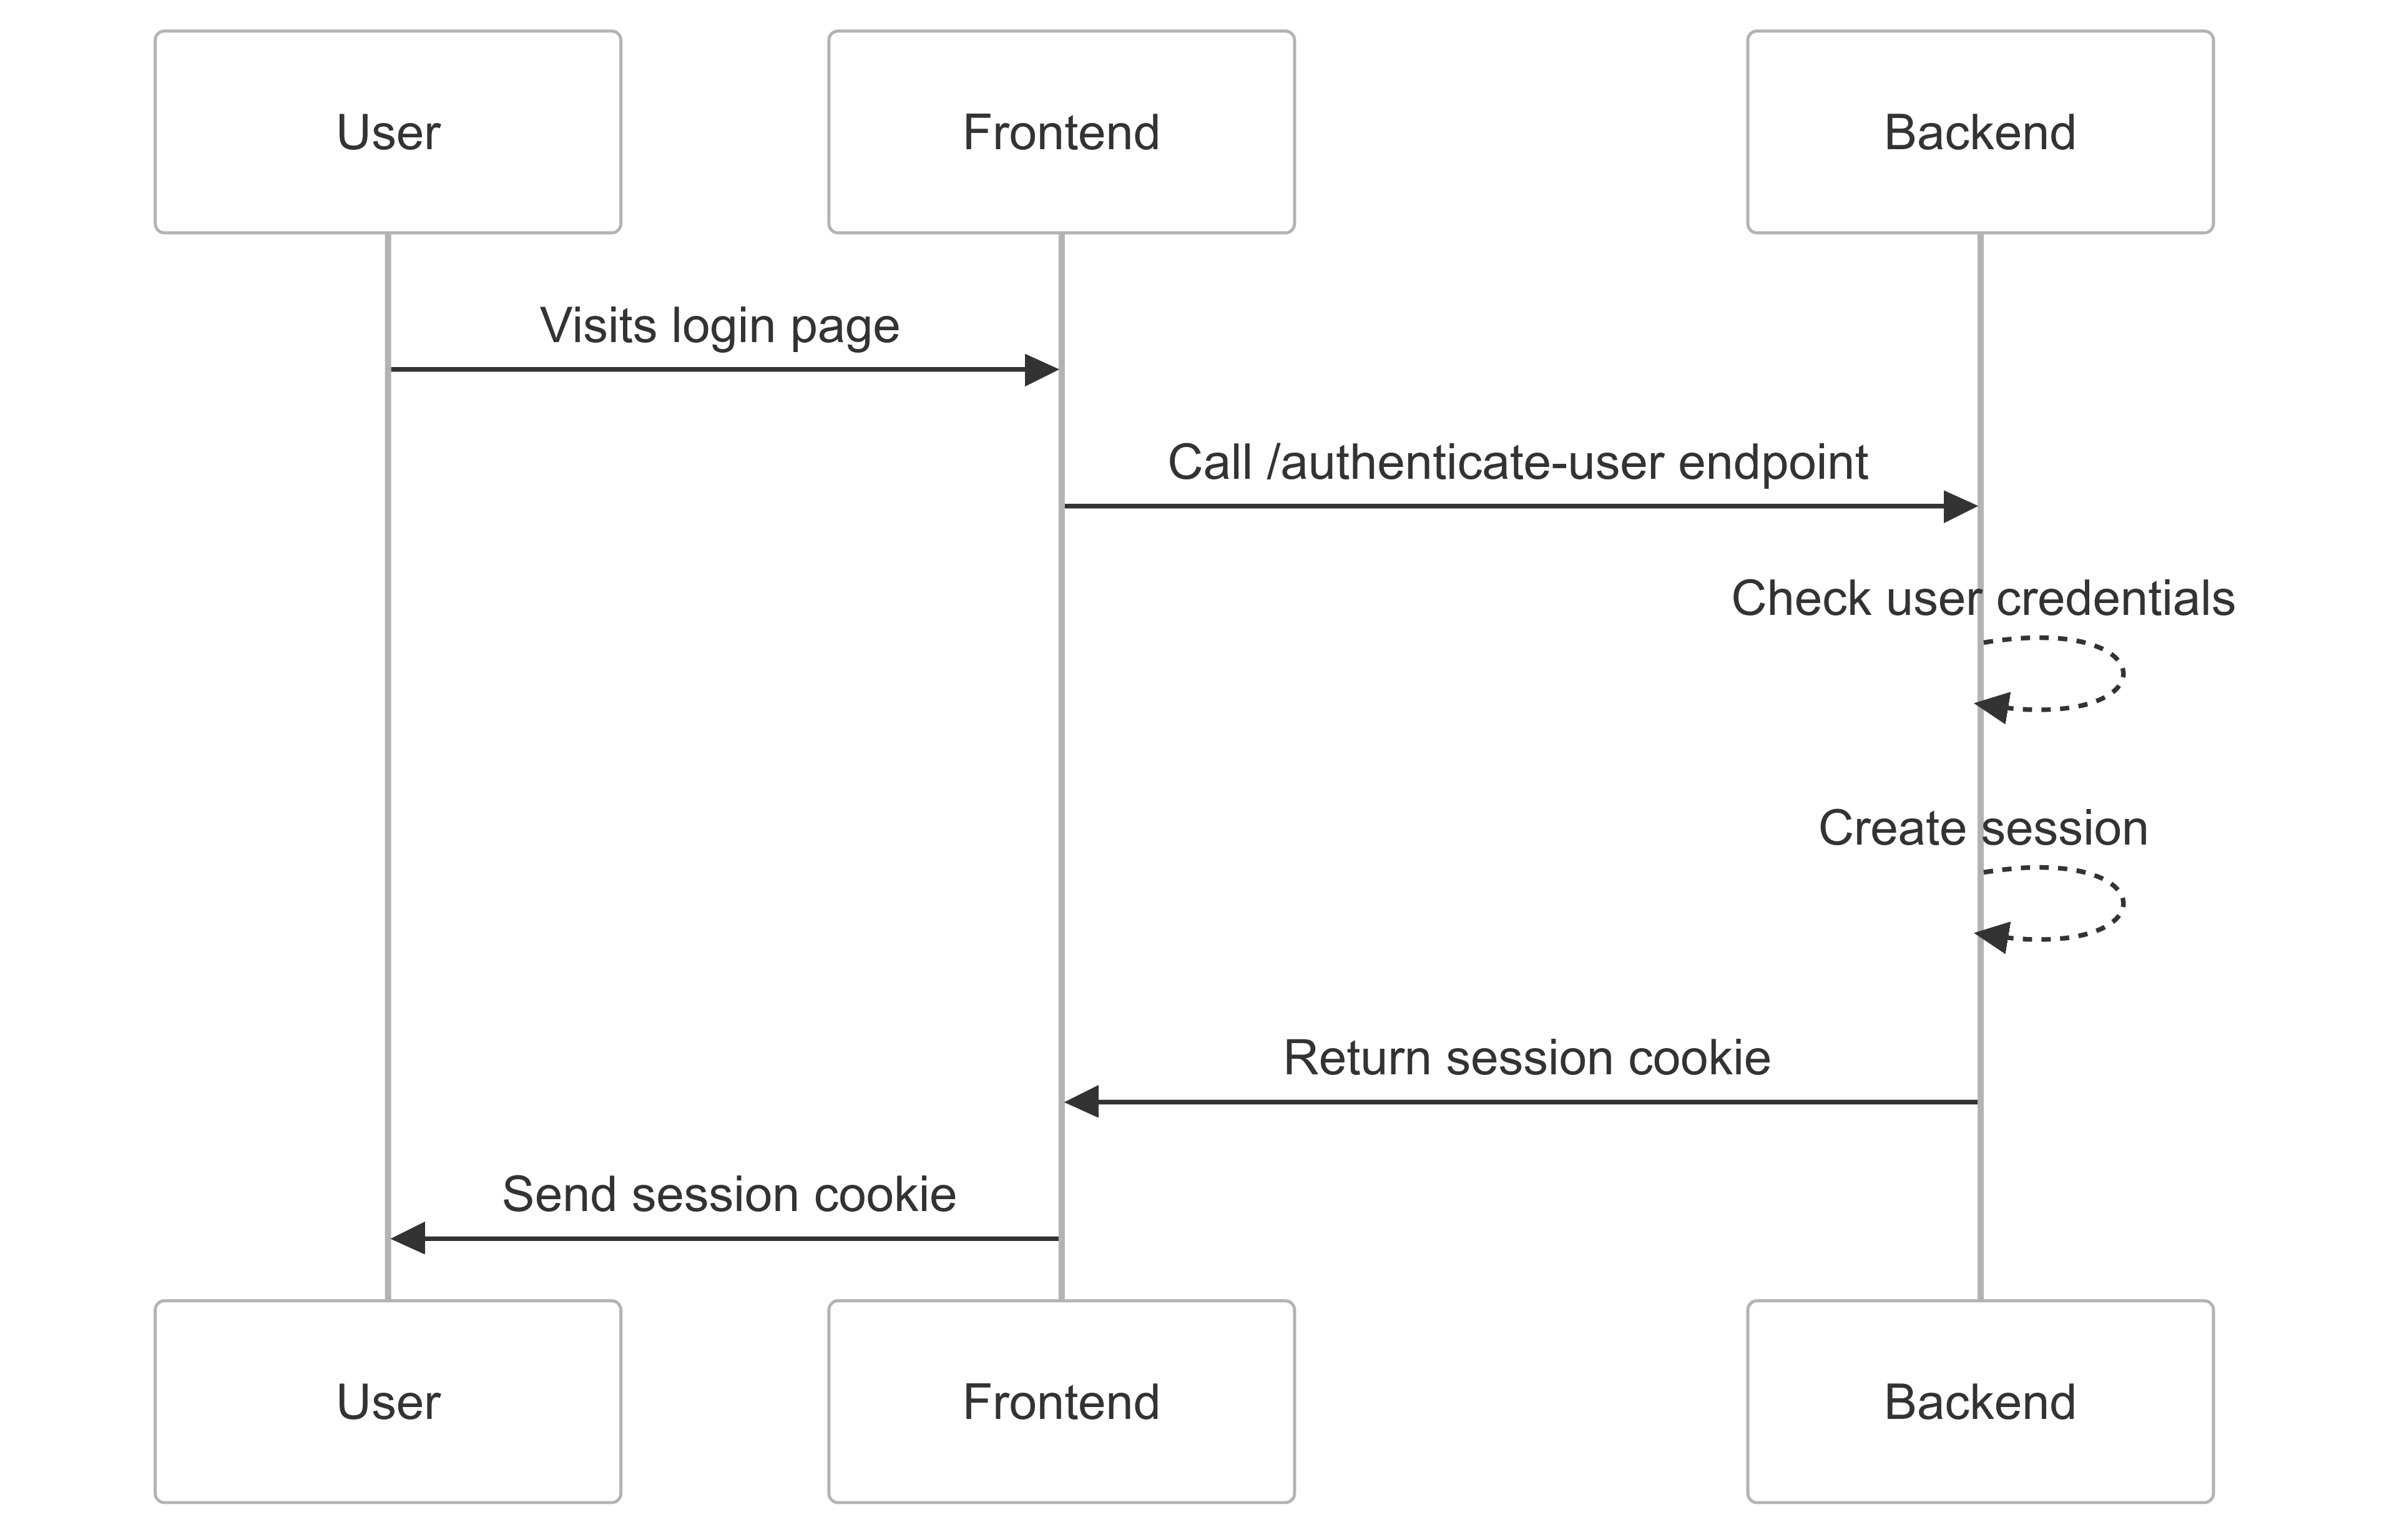
\includegraphics[width=0.9\textwidth, keepaspectratio]{figures/authentication-sequence.png}
    \caption{Login flow with session cookies}
    \label{fig:authentication-sequence}
\end{figure}

\subsubsection{Input validation and sanitization}

Input validation is a method of checking the incoming data for the proper format and allowable values and meeting the given constraints. It is a pillar of security. Frameworks usually can check the general properties of a request, such as whether the input is expected in JSON format, which is JSON and has the desired fields. Enforcing more specific rules, such as user name requirements, that vary based on the business logic and specific use cases may require manual or automatic checks performed with specialized libraries and functions.

The presentation layer, specifically the API handlers, is responsible for validation and sanitization in the platform. The framework and Go standard library help verify the JSON format and URL params, and the handler code performs the other checks. These codes follow the practice of returning an error immediately when a validation fails. This practice prevents the continuing execution of forbidden business logic while keeping the state consistent. Listing~\ref{lst:validation-example} shows an example of validations performed on a quiz session submission.

\begin{lstlisting}[caption=Validation example,label=lst:validation-example]
    // Get the quiz session for the given ID
    quizSession, err := sqlcQuerier.GetQuizSession(
        ctx,
        quizSessionId,
    )
    if err != nil {
        return echo.NewHTTPError(http.StatusNotFound, fmt.Sprintf("quiz session '%s' is not found", quizSessionId))
    }

    // Check the session is finished
    if quizSession.FinishedAt.Valid {
        return echo.NewHTTPError(http.StatusConflict, fmt.Sprintf("quiz session '%s' is already submitted", quizSessionId))
    }

    // Check the user is trying to finished someones session
    if quizSession.UserID != userId {
        return echo.NewHTTPError(http.StatusForbidden, "cannot submit other user's quiz session")
    }
\end{lstlisting}

\subsubsection{SQL injection prevention}

SQL injection is a code injection technique that aims to access and modify unauthorized database data with carefully crafted queries. During this attack, the attacker tries to guess the SQL queries used by the application and then modify them through improperly validated inputs. Preventing this kind of attack is complicated due to the endless possibilities of inputs. Usually, the SQL libraries and Object Relational Mapping (ORM) software help the developers defend against it. The two SQL libraries I used do it differently; SQLx offers solutions for creating prepared statements, while SQLc generates code containing prepared statements.

\section{AI integration Design}

The AI features of the platform are integrated into the \texttt{LLM API} or the server that Máté calls NLP-Service\texttt{NLP-Service}NLP-Service. It is a small Python-based web server that provides the platform with question generation and context chunking capabilities. This component is entirely designed and implemented by Máté. One of his main design goals was to make this service expandable by providing an easy way to integrate different AI models.

\subsection{Component architecture}

Figure~\ref{fig:nlp-service-component} shows the components of the NLP-Service. The service provides four endpoints: one for chunking the long user context and 3 for generating questions for these types: single choice, multiple choice, and boolean questions. The service consists of these modules: \texttt{LLM-IO} for managing the question creation, \texttt{Lang-detect} for detecting the context's language, \texttt{Chunking} for chunking the text, and the LLM providers for making a unified interface for \texttt{LLM-IO} to communicate with the models.

\begin{figure}[H]
    \centering
    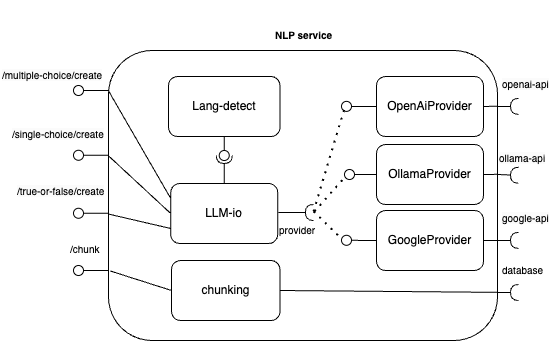
\includegraphics[width=0.8\textwidth, keepaspectratio]{figures/nlp-service-component.png}
    \caption{Components of the NLP service, made by: Máté Debreczeni}
    \label{fig:nlp-service-component}
\end{figure}

\subsection{Example request and response}

Listing~\ref{lst:nlp-service-question-generation} shows an example HTTP request and its response for a multiple-choice question generation.

\begin{lstlisting}[caption=Validation example,label=lst:nlp-service-question-generation]
--- Request:

POST /multiple-choice/create HTTP/1.1
Host: llm-api.spacedace.orb.local:80
Content-Type: application/json
Content-Length: 134

{
  "prompt": "Napjainkban az összes Linux tűzfal alapját a 2001-ben megjelent, 2.4-es Linux kernel részét képezi netfilter képezi."
}

--- Response:

HTTP/1.1 200 OK
date: Mon, 02 Dec 2024 19:37:14 GMT
server: uvicorn
content-length: 392
content-type: application/json

{"question":"Melyik állítás igaz a Linux tűzfalakkal kapcsolatban a megadott kontextus alapján?","options":["A Linux tűzfalak alapja a 2001 előtti Linux kernel.","A netfilter a 2.4-es Linux kernel része, és a Linux tűzfalak alapját képezi.","A netfilter egy 2001 után fejlesztett tűzfal technológia.","A Linux tűzfalak nem használják a netfiltert."],"correct_options":["B"]}

\end{lstlisting}

\subsection{Endpoint overview}

The following table~\ref{tab:nlp-service-endpoints} lists the available endpoint of the NLP-Service. Three endpoints for question generation receive a context chunk, and the service creates a prompt after detecting the language of the given text. It sends a request to the configured LLM, waits for its response to validate it, and sends it back to the caller. However, the chunking endpoint processes the text locally. It saves the chunks to the database and responds to the caller with the list of chunks and IDs.

\begin{table}[H]
    \begin{tabular}{|l|l|l|}
        \hline
        \textbf{URL} & \textbf{Method} & \textbf{Description} \\
        \hline
        /chunk & POST & Generate smaller text chunks from the given context\\
        \hline
        /single-choice/create & POST & Generates a single choice question \\
        \hline
        /true-or-false/create & POST & Generates a multiple choice question \\
        \hline
        /true-or-false/create & POST & Generates a boolean question \\
        \hline
    \end{tabular}
    \caption{NLP-Service endpoint overview}
    \label{tab:nlp-service-endpoints}
\end{table}